\documentclass[11pt,a4paper]{article}

\usepackage[margin=2.4cm]{geometry}
\usepackage[T1]{fontenc}
\usepackage[utf8]{inputenc}
\usepackage{lmodern}
\usepackage{microtype}
\usepackage{amsmath,amssymb}
\usepackage{graphicx}
\usepackage{booktabs}
\usepackage{siunitx}
\usepackage{caption}
\usepackage{subcaption}
\usepackage{float}
\usepackage{xcolor}
\usepackage[hidelinks]{hyperref}
\usepackage[numbers,sort&compress]{natbib}

\graphicspath{{figures/}}

\sisetup{
  separate-uncertainty=true,
  per-mode=symbol
}

\newcommand{\Bplus}{\ensuremath{B^+}}
\newcommand{\Bminus}{\ensuremath{B^-}}
\newcommand{\ACP}{\ensuremath{A_{\mathrm{CP}}}}
\newcommand{\mevcc}{\ensuremath{\mathrm{MeV}/c^2}}
\newcommand{\gevfour}{\ensuremath{\mathrm{GeV}^2/c^4}}

\title{\textbf{A CERN Open Data Analysis of Three-Body B-Meson Decays}\\
\large Invariant-Mass Reconstruction, Signal Classification, CP-Asymmetry Diagnostics, and Dalitz-Plot Studies}
\author{Yanis Idir\\
\small Portfolio report for experimental particle-physics PhD applications}
\date{\today}

\begin{document}
\pagenumbering{gobble}

\begin{titlepage}
  \centering
  \vspace*{2.0cm}
  {\Large \textsc{LHCb Open Data Analysis}\par}
  \vspace{1.2cm}
  {\huge\bfseries A CERN Open Data Analysis of Three-Body B-Meson Decays\par}
  \vspace{0.5cm}
  {\Large Invariant-Mass Reconstruction, Signal Classification, CP-Asymmetry Diagnostics, and Dalitz-Plot Studies\par}
  \vspace{1.8cm}
  {\large Yanis Idir\par}
  \vspace{0.2cm}
  {\small Portfolio report for experimental particle-physics PhD applications\par}
  \vfill
  \begin{abstract}
  This report presents a compact but realistic high-energy-physics analysis workflow based on LHCb CERN Open Data. Three-body B-meson candidates are reconstructed from charged-hadron tracks under a kaon mass hypothesis. The workflow uses ROOT input files, Python-based columnar data processing, invariant-mass reconstruction, event selection, a sideband-labelled Random Forest classifier, a raw charge-asymmetry diagnostic, and Dalitz-plot visualisations. The report emphasizes reproducibility, modular scientific code, and analysis reasoning suitable for an early-stage experimental particle-physics project.
  \end{abstract}
  \vfill
  {\large \today\par}
\end{titlepage}

\clearpage
\pagenumbering{roman}
\tableofcontents
\clearpage
\pagenumbering{arabic}

\section{Introduction}

The Standard Model of particle physics describes the known elementary particles and their interactions with remarkable precision. Nevertheless, several observed features of the Universe remain only partially understood. One of the most important is the matter--antimatter asymmetry: cosmological observations indicate that the visible Universe is dominated by matter, while the known laws of particle physics contain only limited sources of charge-parity (CP) violation. In the Standard Model, CP violation arises from a single complex phase in the quark-mixing matrix~\cite{ckm,km}, and the size of the resulting effects is far too small to account for the observed baryon asymmetry. Precision studies of flavour-changing processes are therefore a central part of modern particle physics.

Flavour physics studies transitions between different quark flavours. In the heavy-flavour sector, hadrons containing beauty quarks provide especially rich laboratories. The large mass of the beauty quark allows many decay modes, including multibody final states in which resonant and non-resonant amplitudes can interfere. Such interference can generate local CP-asymmetric effects in restricted regions of phase space, even when the integrated asymmetry is small.

B mesons are bound states containing a beauty quark or antiquark and a lighter valence quark. Charged B mesons, denoted \Bplus{} and \Bminus{}, form a natural pair of charge-conjugate systems. By comparing the observed yields or distributions of \Bplus{} and \Bminus{} candidates, one can construct raw asymmetry observables. In a simplified counting analysis, the integrated asymmetry is written as
\begin{equation}
  \ACP^{\mathrm{raw}} =
  \frac{N(\Bminus) - N(\Bplus)}
       {N(\Bminus) + N(\Bplus)} ,
  \label{eq:acp_intro}
\end{equation}
where $N(\Bplus)$ and $N(\Bminus)$ are observed candidate counts. A full physics measurement must correct this raw quantity for background contributions, detector-induced charge asymmetries, production asymmetries, trigger effects, and selection efficiencies. The present project treats Eq.~\ref{eq:acp_intro} as an analysis diagnostic rather than as a final CP-violation measurement.

This report documents a reproducible analysis workflow built with CERN Open Data~\cite{cernopendata}. The project focuses on a sample of reconstructed LHCb three-hadron B candidates stored in ROOT files. The analysis reconstructs the B-candidate invariant mass, applies simple physics-motivated selections, fits the mass peak, trains a signal/background classifier using sideband labels, separates charge-conjugate candidates, and produces Dalitz-plot distributions. The goal is to demonstrate a modern high-energy-physics (HEP) workflow using transparent scientific reasoning and modular Python code.

The analysis is intentionally compact. It is not presented as a publishable LHCb measurement, but as a polished student-level project that mirrors the structure of a real experimental analysis: data access, reconstruction, selection, modelling, validation plots, and interpretation of limitations. This makes it suitable as a technical portfolio project for applications in experimental particle physics.

\section{The LHCb Experiment}

The Large Hadron Collider beauty experiment (LHCb) is a forward spectrometer at the CERN Large Hadron Collider designed for precision studies of hadrons containing beauty and charm quarks~\cite{lhcbdetector}. Proton--proton collisions at the LHC produce heavy quarks predominantly in the forward and backward regions. LHCb exploits this production topology by covering a forward angular region, providing excellent tracking, vertexing, momentum resolution, and particle identification.

The detector design is particularly well suited to heavy-flavour analyses. B hadrons have lifetimes long enough to travel measurable distances before decaying. This displaced-decay topology is identified by reconstructing primary vertices from the proton--proton interaction and secondary vertices from the B-hadron decay products. The distance between these vertices and the quality of the reconstructed secondary vertex are powerful handles for suppressing prompt combinatorial background.

Charged-particle tracking is performed with a system of silicon and tracking stations around a dipole magnet. The curvature of charged-particle trajectories in the magnetic field provides a momentum measurement and determines the charge sign. In the present analysis, the track momentum components are used directly to build four-vectors for the three daughter hadrons. The charge information is used later to classify candidates as \Bplus{} or \Bminus{}.

Particle identification (PID) is another central ingredient. LHCb uses ring-imaging Cherenkov detectors to distinguish kaons, pions, and protons over a broad momentum range. The open-data ntuples used in this project contain per-track PID-related variables such as kaon and pion probability-like observables. A simple kaon-PID selection is applied to build a clean demonstration sample under a $B \to K K K$ mass hypothesis.

In a complete LHCb analysis, detector effects are modelled with simulation, calibration samples, and data-driven corrections. This project keeps the detector treatment deliberately simple, but it preserves the main conceptual ingredients: displaced B vertices, charged-track reconstruction, particle identification, and magnet-polarity awareness.

\section{Dataset and Software Framework}

\subsection{ROOT input files}

The project uses the CERN Open Data record \emph{Matter Antimatter Differences
(B meson decays to three hadrons)}~\cite{b2hhhdata}, released by the LHCb
collaboration in 2017 under a CC0 licence. The record contains three ROOT files
with reconstructed $B$-candidate ntuples. The two data files,
\begin{center}
  \texttt{data/raw/B2HHH\_MagnetDown.root}, \qquad
  \texttt{data/raw/B2HHH\_MagnetUp.root},
\end{center}
hold the same data-taking period recorded with the two polarities of the LHCb
dipole magnet; the third, \texttt{PhaseSpaceSimulation.root}, is kept for the
extensions discussed in Sec.~\ref{sec:conclusion}. Both polarities are used for
the raw asymmetry. Reversing the magnetic field swaps the side of the detector
towards which each charge is bent, so averaging the two polarities cancels
left--right detection asymmetries to first order
(Sec.~\ref{sec:cp}); MagnetUp also provides an independent sample on which a
feature seen in MagnetDown can be checked. The selection, the classifier study and
the exploratory notebooks were developed on MagnetDown.

The data are stored in the ROOT format~\cite{root}, a standard file and object format in high-energy physics. The relevant event information is contained in a tree named \texttt{DecayTree}. A ROOT \texttt{TTree} stores columnar data: each branch corresponds to one observable, such as a momentum component, charge, PID response, vertex quality, or flight distance. This format is efficient for large event samples because only the branches needed for a given analysis step need to be read.

\subsection{Python analysis workflow}

The analysis is implemented as a Python workflow. Reusable functions live under \texttt{src/}; exploratory notebooks under \texttt{notebooks/}; the fit entry points under \texttt{scripts/}; and the toy-MC, systematic, charge-shape and Dalitz studies under \texttt{studies/}. Every study writes its numerical output as JSON and CSV under \texttt{results/}, so each number quoted in this report can be traced to the file that produced it. The main software components are listed in Table~\ref{tab:software}; they are drawn from the scientific Python stack~\cite{numpy,matplotlib} and from the Scikit-HEP ecosystem~\cite{scikithep}.

\begin{table}[H]
  \centering
  \caption{Main software tools used in the analysis workflow.}
  \label{tab:software}
  \begin{tabular}{ll}
    \toprule
    Tool & Role in the analysis \\
    \midrule
    ROOT & Standard HEP file format and ntuple storage \\
    \texttt{uproot} & Reading ROOT TTrees directly in Python \\
    \texttt{pandas} & Tabular event manipulation and selections \\
    \texttt{numpy} & Vectorised numerical calculations \\
    \texttt{scipy} & Special functions used in the mass models \\
    \texttt{iminuit} & \textsc{Minuit} interface for the likelihood minimisation \\
    \texttt{matplotlib} & Publication-style figures \\
    \texttt{scikit-learn} & Random Forest classifier and performance metrics \\
    \bottomrule
  \end{tabular}
\end{table}

The branch set used throughout the analysis includes the momentum components \texttt{H1\_PX}, \texttt{H1\_PY}, \texttt{H1\_PZ} through \texttt{H3\_PZ}, the three track charges, PID variables such as \texttt{H1\_ProbK}, and B-candidate quality variables such as \texttt{B\_VertexChi2} and \texttt{B\_FlightDistance}. A shared selection helper loads these branches, reconstructs the B-candidate mass, and applies the common baseline cuts. This avoids duplicated logic between the mass, machine-learning, CP-asymmetry, and Dalitz notebooks.

The workflow is intentionally modular. The main reusable components are the invariant-mass reconstruction module \path{src/reconstruction/invariant_mass.py}, the mass models and likelihood fit in \path{src/fitting/}, the shared selection in \path{src/physics/selection.py}, the Dalitz-kinematics module \path{src/physics/dalitz.py}, the plotting helpers in \path{src/plotting/mass_plots.py}, and the classifier utilities in \path{src/ml/signal_background.py}. This separation mirrors the structure of a maintainable HEP analysis, where physics definitions, fit models, plotting conventions and machine-learning utilities are reusable across studies rather than duplicated in each of them.

\section{Invariant Mass Reconstruction}

\subsection{Relativistic mass formula}

The key reconstructed observable is the invariant mass of the three-hadron B candidate. For a system of particles with total energy $E$ and total momentum $\vec{p}$, the invariant mass is defined by
\begin{equation}
  m^2 c^4 = E^2 - |\vec{p}|^2 c^2 .
\end{equation}
In high-energy-physics units with $c=1$, this becomes
\begin{equation}
  m^2 = E^2 - p_x^2 - p_y^2 - p_z^2 .
  \label{eq:invariant_mass}
\end{equation}

For each daughter track, the analysis uses a charged-kaon mass hypothesis,
\begin{equation}
  m_K = \SI{493.677}{\mega\electronvolt}/c^2 ,
\end{equation}
and reconstructs the energy as
\begin{equation}
  E_i = \sqrt{p_{x,i}^2 + p_{y,i}^2 + p_{z,i}^2 + m_K^2}.
\end{equation}
The B-candidate four-vector is then the sum of the three daughter four-vectors:
\begin{equation}
  E_B = \sum_{i=1}^{3} E_i, \qquad
  \vec{p}_B = \sum_{i=1}^{3} \vec{p}_i .
\end{equation}
Substituting these quantities into Eq.~\ref{eq:invariant_mass} gives the reconstructed B-candidate mass. The calculation is performed event-by-event with vectorised \texttt{numpy} operations.

\subsection{Mass spectrum before and after selection}

Figure~\ref{fig:mass_before} shows the reconstructed three-kaon mass spectrum before the baseline event selection. The distribution contains a broad combinatorial component as well as a visible accumulation near the expected B-meson mass region. This broad structure is typical of a preselection-level hadron-collider sample, where many random track combinations can satisfy a loose candidate definition.

\begin{figure}[H]
  \centering
  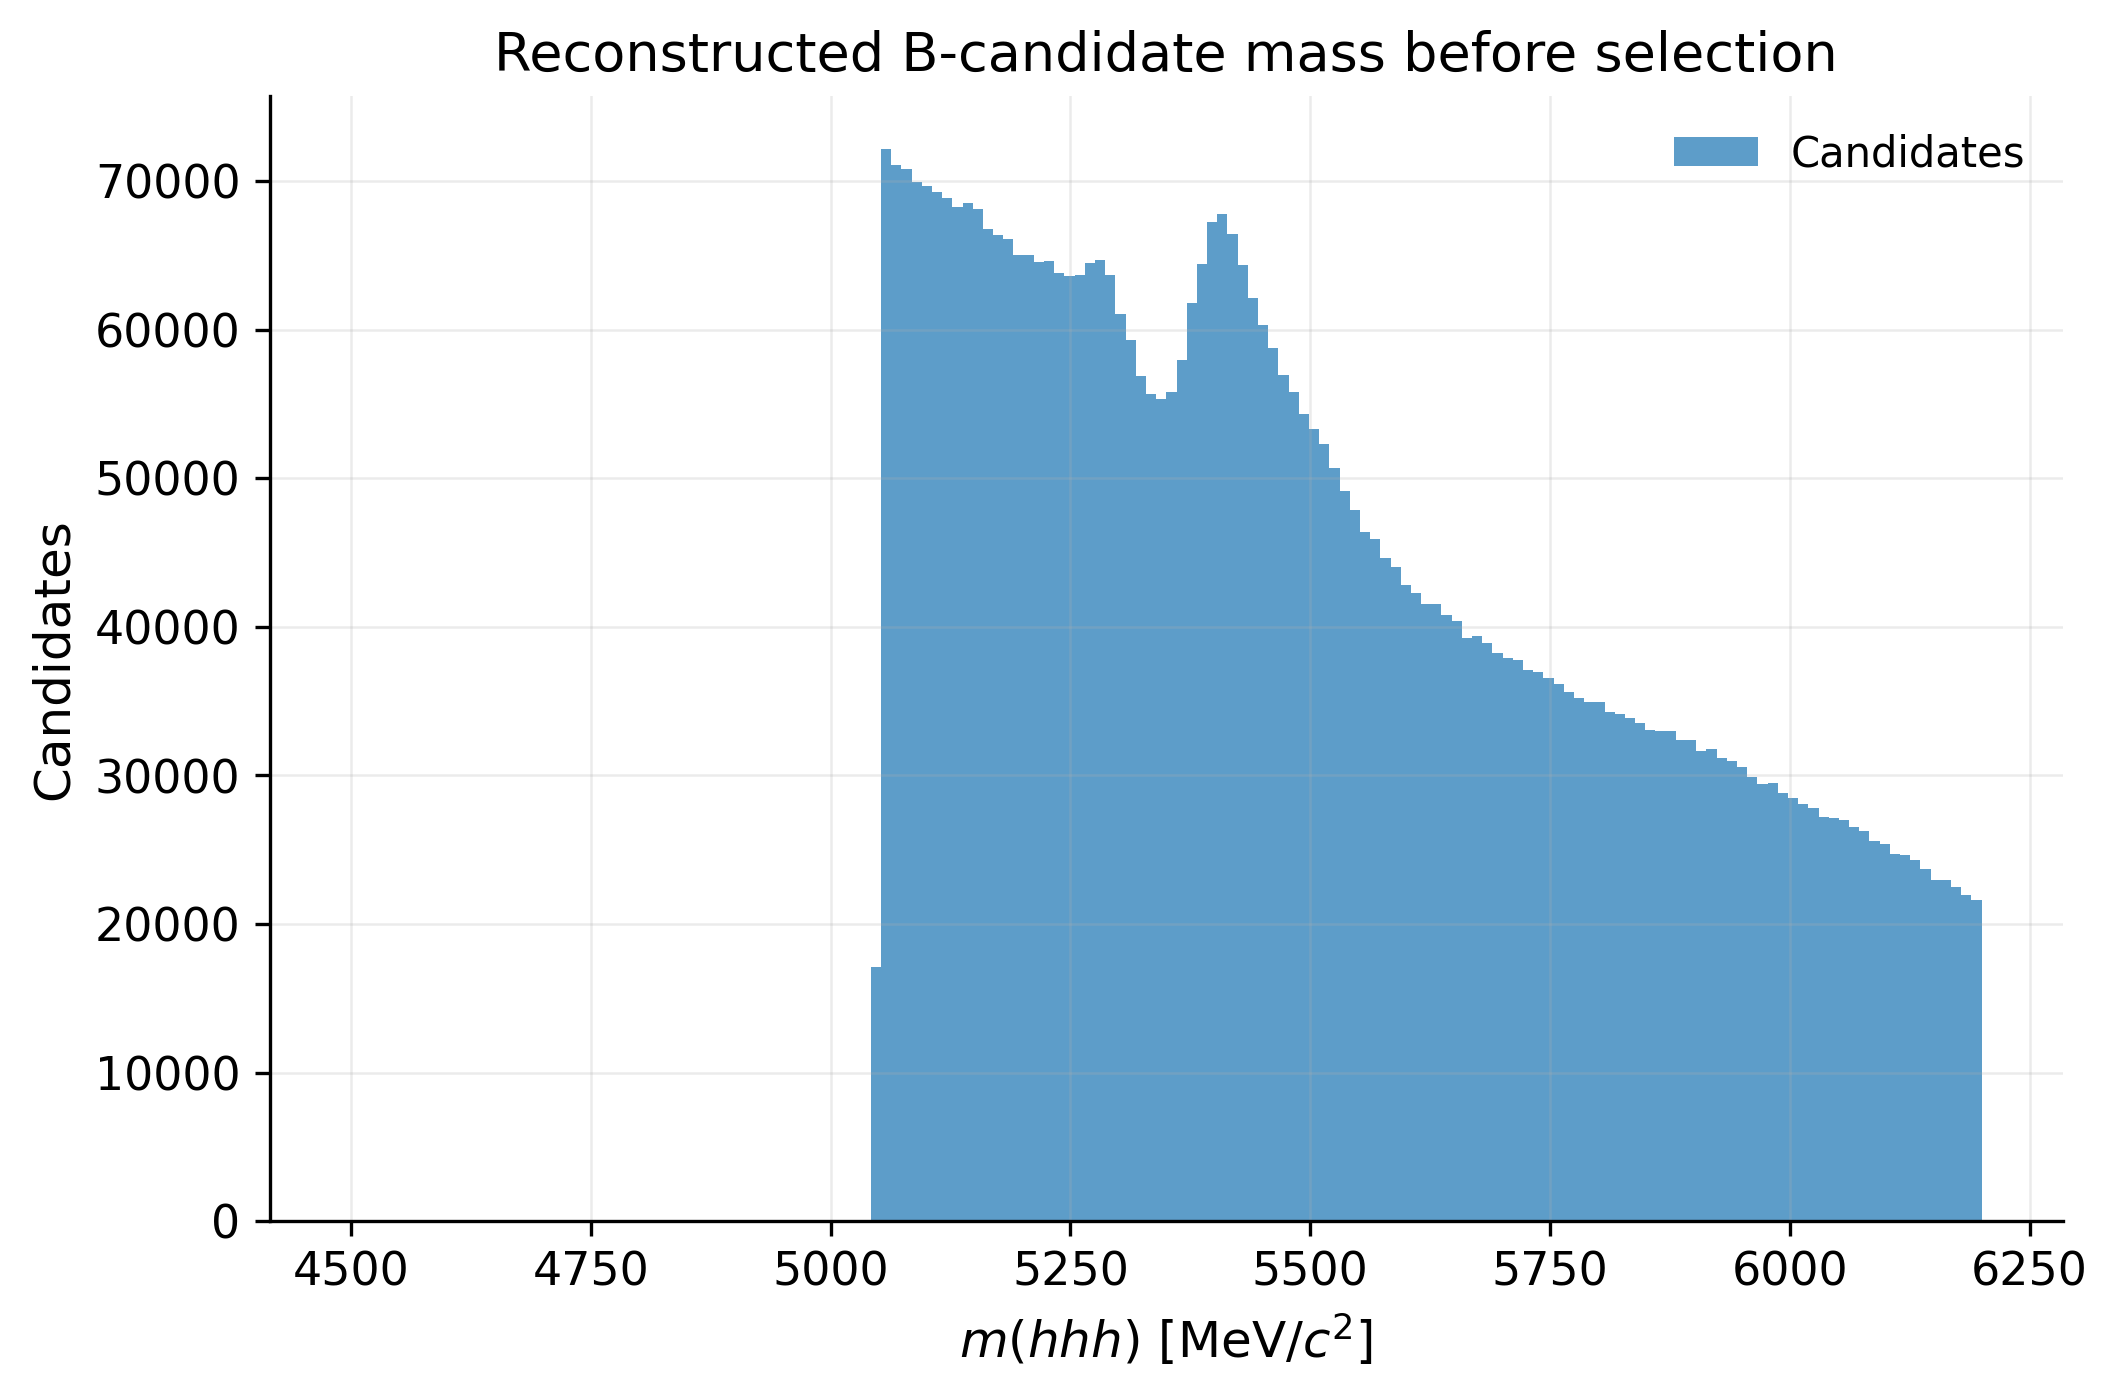
\includegraphics[width=0.82\textwidth]{B_mass_before_cuts.png}
  \caption{Reconstructed B-candidate invariant-mass distribution before baseline selection.}
  \label{fig:mass_before}
\end{figure}

After applying quality, displacement, and kaon-PID selections, the mass spectrum becomes visibly cleaner, as shown in Fig.~\ref{fig:mass_after}. The selection enhances the relative contribution of candidates compatible with a displaced B decay and suppresses a large fraction of combinatorial background.

\begin{figure}[H]
  \centering
  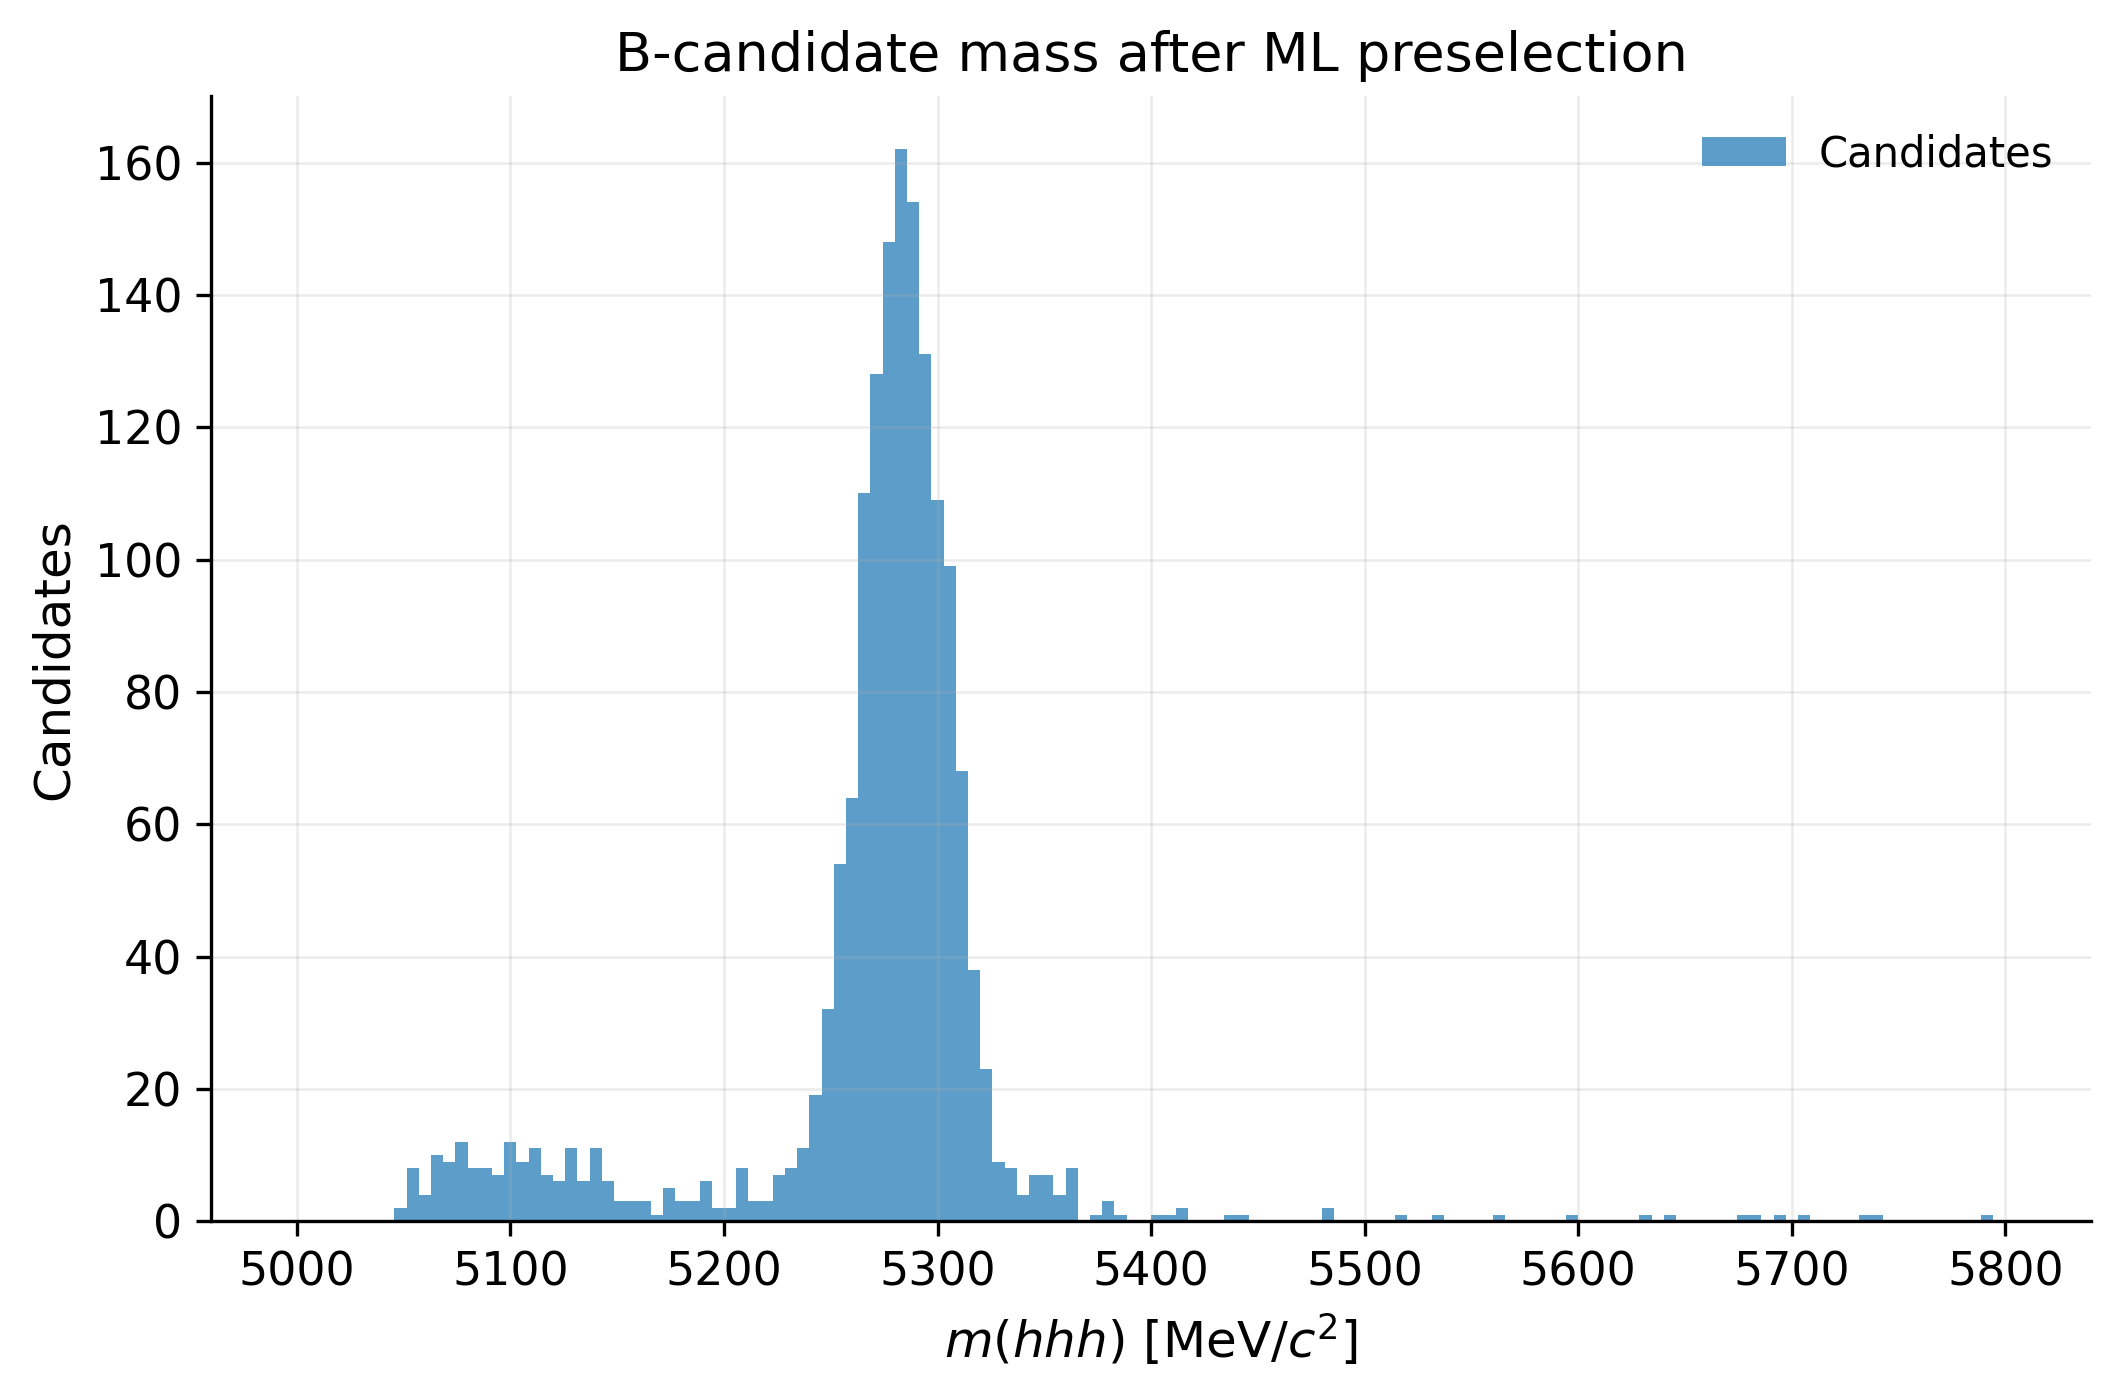
\includegraphics[width=0.82\textwidth]{B_mass_after_cuts.png}
  \caption{Reconstructed B-candidate invariant-mass distribution after baseline physics selections.}
  \label{fig:mass_after}
\end{figure}

\subsection{Signal-plus-background fit}
\label{sec:mass_fit}

A nominal signal extraction is performed with an extended binned maximum-likelihood
fit of the model
\begin{equation}
  f(m) =
  N_s S(m) + N_b B(m) ,
  \label{eq:mass_fit_model}
\end{equation}
where $S(m)$ is the signal mass shape, $B(m)$ a finite-range exponential
describing the combinatorial background, and $N_s$ and $N_b$ the fitted yields
inside the fitted interval. The likelihood is minimised with
\textsc{Minuit}~\cite{minuit} through the \texttt{iminuit} interface.

Two choices define the nominal configuration, and both are worth stating
explicitly because they are where this analysis is most fragile.

\paragraph{Fitted interval.} The fit is performed over
$5200 < m(hhh) < 5600~\mevcc$. The ntuple itself starts at $5050~\mevcc$, and
the spectrum between $5050$ and about $5180~\mevcc$ holds a structure that the
combinatorial background model does not describe. It is the same for the two
charges, and it falls off at the kinematic limit $m_B - m_\pi \approx
5140~\mevcc$ of a $B$ decay in which a pion is not reconstructed, smeared by the
resolution: the signature of partially reconstructed decays. An ARGUS shape with
that endpoint, convolved with the resolution, was tried over the full
$5050$--$5600~\mevcc$ range, but the ntuple boundary leaves only the top of the
shape visible and its curvature runs to the limit of its allowed range. Starting
the fit at $5200~\mevcc$ removes the region at the cost of a shorter low-mass
sideband.

\paragraph{Signal shape.} The nominal signal shape is a single Gaussian. A
common-mean double Gaussian was tested as the nominal shape, since detector-level
mass peaks often show a narrow core with broader tails, but on this sample its
wide component, $\sigma = 55 \pm 10~\mevcc$, takes over the combinatorial
background: the fitted background yield falls from $180 \pm 21$ to $63 \pm 39$
candidates, and the uncertainty on the signal yield inflates from $52$ to $63$.
The fit does reach a valid minimum, with a narrow-core fraction of
$0.91 \pm 0.03$, once several starting points are tried, but with a truncated
low-mass sideband the data cannot tell a broad resolution tail from the
background. The double Gaussian is therefore used as a systematic variation
rather than as the nominal shape.

The nominal fit of all selected candidates, both charges and both polarities
together, is shown in Fig.~\ref{fig:mass_fit}. Of the $2939$ selected candidates
($1645$ MagnetDown, $1294$ MagnetUp), $2573$ fall inside the fitted interval. The
results are
\begin{align}
  N_s &= 2394 \pm 52, \\
  N_b &= 180 \pm 21, \\
  \mu &= 5284.7 \pm 0.4~\mevcc, \\
  \sigma &= 19.5 \pm 0.4~\mevcc,
\end{align}
with $\chi^2/\mathrm{ndof}=0.74$. Fitted separately, the two polarities give the
same peak position and resolution within $0.1~\mevcc$. The fitted peak position lies within a few
$\mevcc$ of the known $B^\pm$ mass~\cite{pdg}, which is the main closure check on
the four-vector reconstruction and the mass hypothesis. The fitted resolution is
a detector resolution convolved with the kaon mass hypothesis, not a measurement
of the natural width.

\begin{figure}[H]
  \centering
  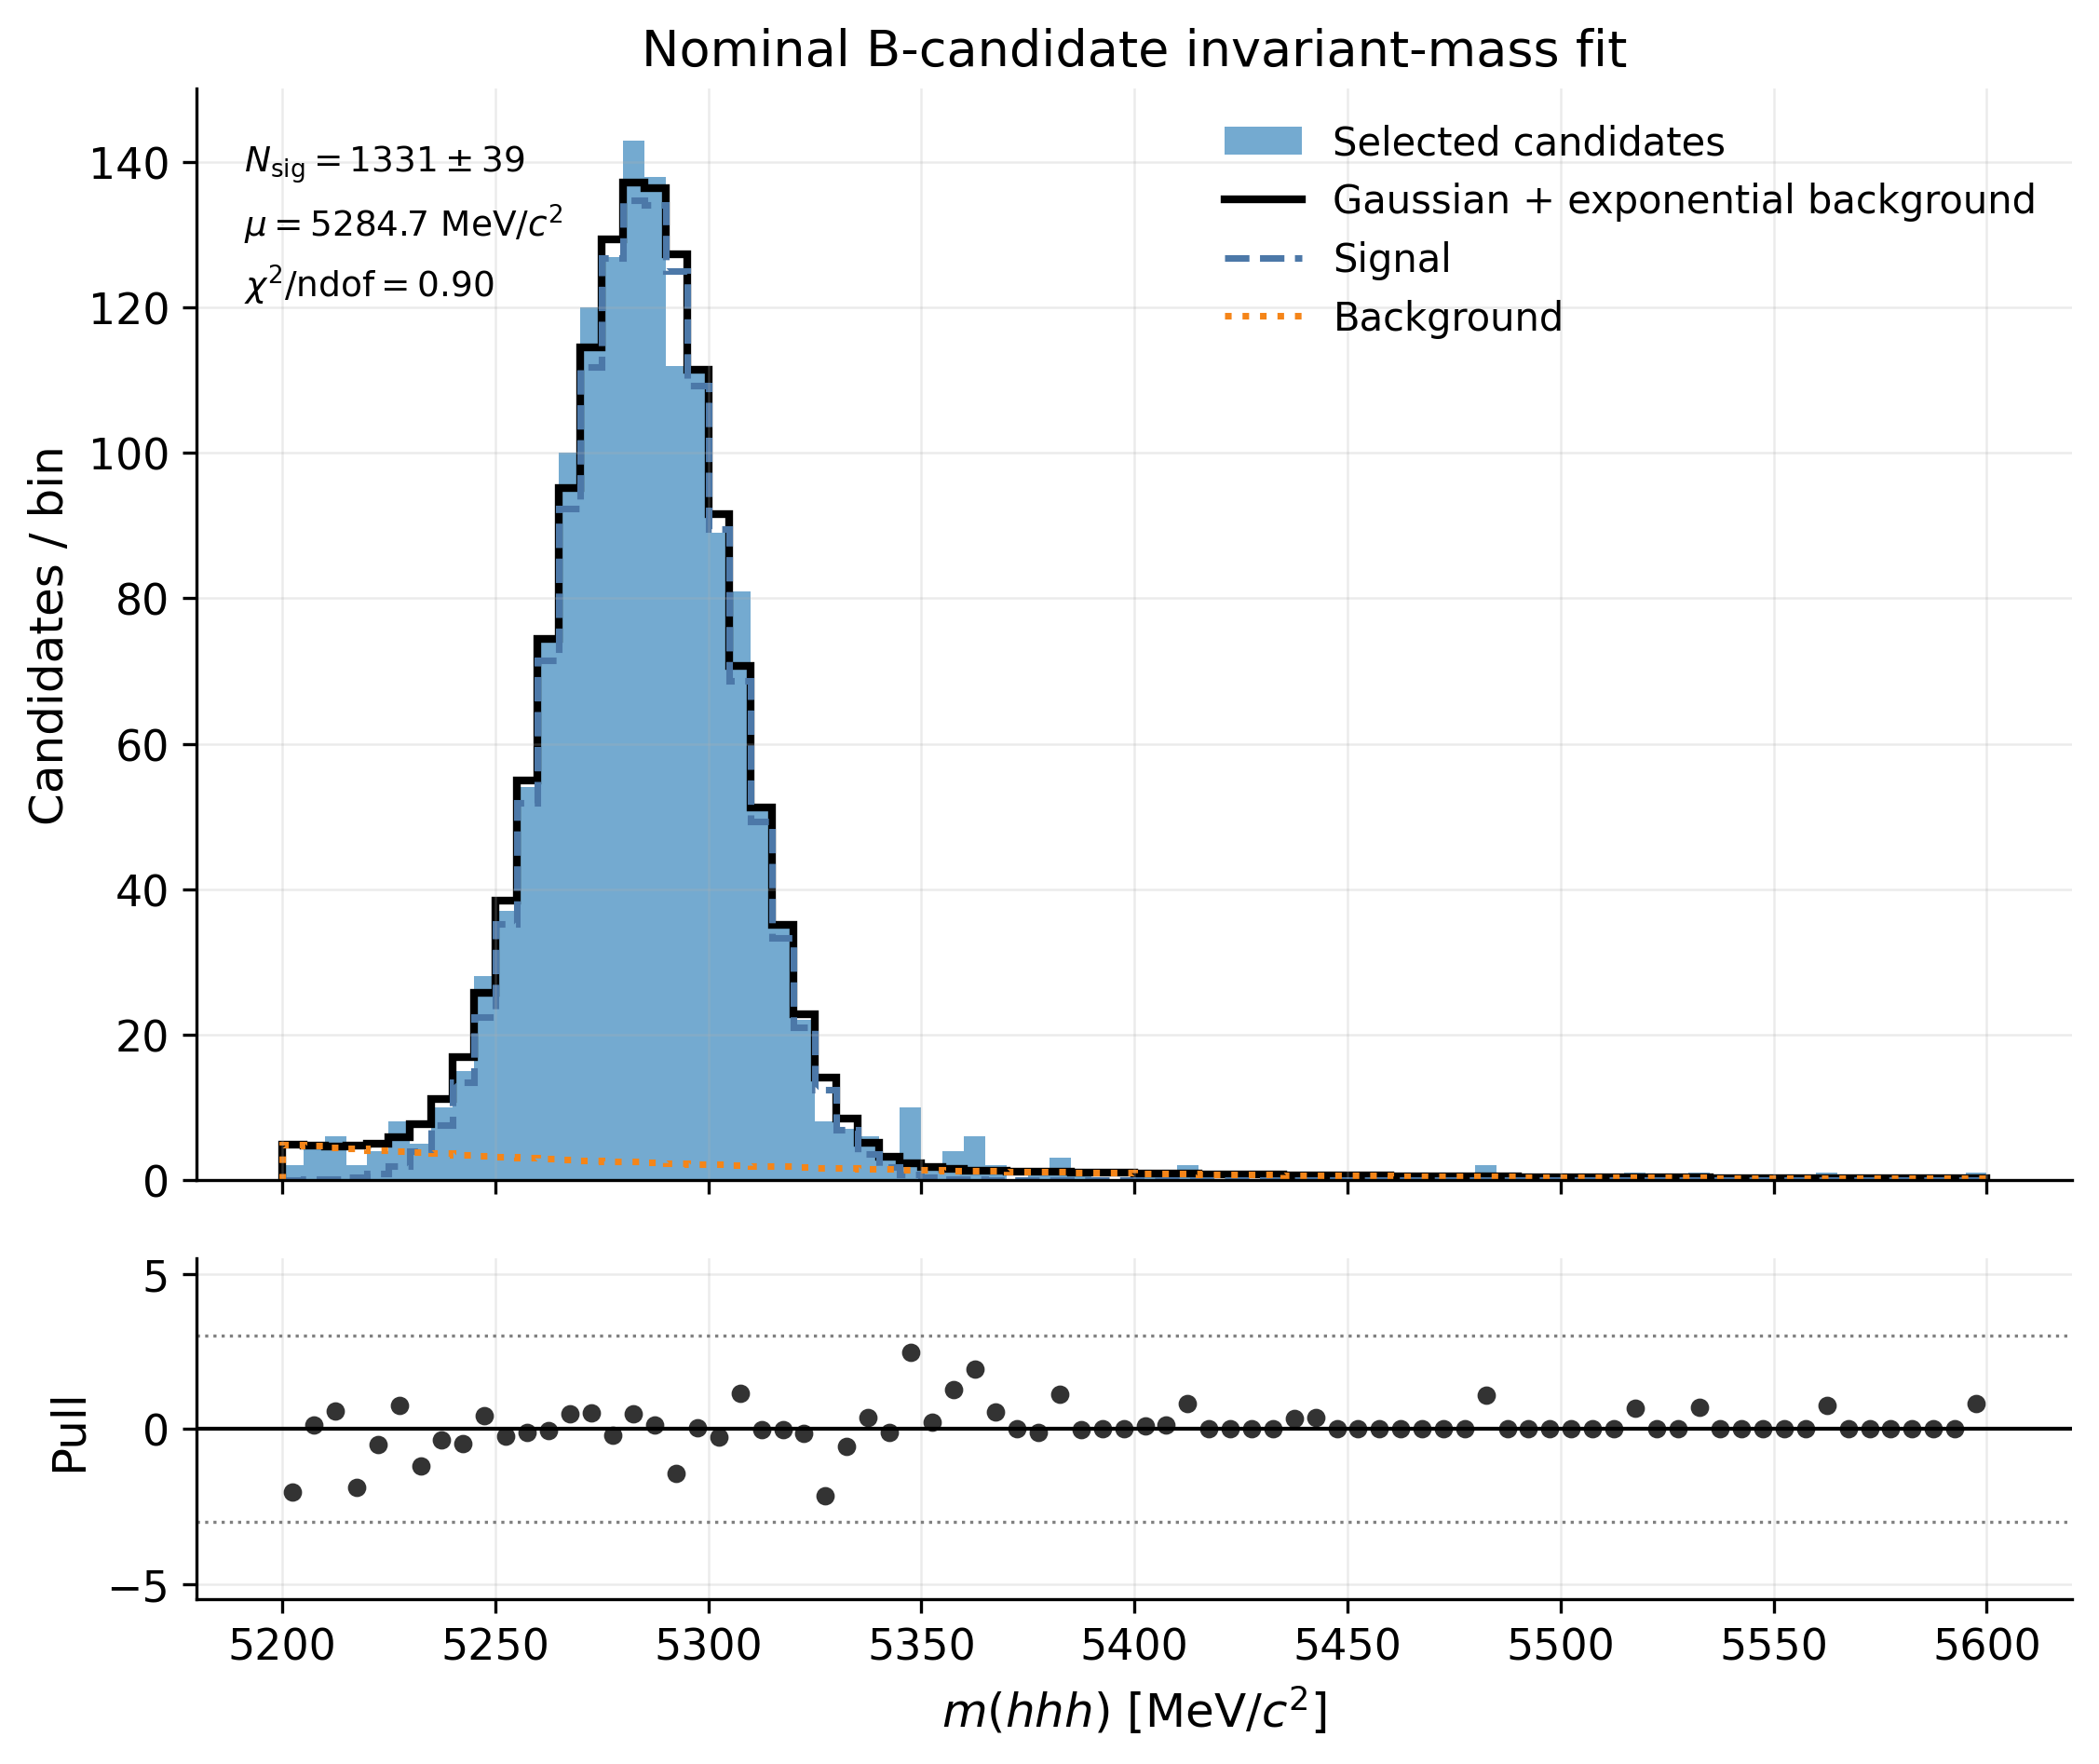
\includegraphics[width=0.82\textwidth]{mass_fit_plot.png}
  \caption{Selected $B$-candidate mass spectrum fitted with a single-Gaussian signal component and a finite-range exponential background, with fit residuals below.}
  \label{fig:mass_fit}
\end{figure}

\section{Event Selection}
\label{sec:selection_effect}

Event selection is a central part of any hadron-collider analysis. The raw candidate sample contains true signal decays, partially reconstructed backgrounds, misidentified backgrounds, and random combinations of charged tracks. The goal of the baseline selection is to retain a useful signal-rich region while keeping the cuts simple enough to interpret.

The open-data ntuple is already preselected: it contains only candidates with
$\chi^2_{\mathrm{vertex}}(B) < 12$ and $d_{\mathrm{flight}}(B) > 3~\mathrm{mm}$.
The baseline selection applied on top of that is
\begin{align}
  \chi^2_{\mathrm{vertex}}(B) &< 5, \\
  d_{\mathrm{flight}}(B) &> 20~\mathrm{mm}, \\
  P_K(H_1), P_K(H_2), P_K(H_3) &> 0.5 .
\end{align}
Here $\chi^2_{\mathrm{vertex}}(B)$ is the $\chi^2$ of the three-track vertex fit,
not divided by its number of degrees of freedom; $d_{\mathrm{flight}}(B)$ is the
reconstructed distance in millimetres between the primary and secondary vertices;
and $P_K(H_i)$ is the kaon PID response for daughter track $H_i$, a
probability-like variable between 0 and 1.

The selection is severe: it keeps $1645$ of the $5\,135\,823$ MagnetDown
candidates and $1294$ of the $3\,420\,295$ MagnetUp ones, a retention of
$3$--$4\times10^{-4}$. That is a deliberate trade of efficiency
for purity, and it has a consequence used later in this report: after these cuts
there is little residual background left for a classifier to separate.

The vertex-quality cut suppresses candidates whose three tracks do not form a well-reconstructed secondary vertex. This is physically motivated because the daughters of a true B decay should originate from a common decay point. A poor vertex fit is more likely to arise from accidental combinations of tracks produced in different processes or from poorly reconstructed tracks.

The flight-distance selection exploits the finite lifetime of B mesons. Because B hadrons travel a measurable distance before decaying, their decay vertices are displaced from the primary proton--proton interaction point. Requiring a sufficiently large flight distance therefore suppresses prompt background combinations that originate near the primary vertex.

The PID selection implements the kaon mass hypothesis used in the invariant-mass reconstruction. Requiring all three tracks to have kaon-compatible PID values improves the consistency of the reconstructed final state. In a more complete analysis, one would optimize PID requirements with calibration samples and evaluate the corresponding efficiency and misidentification rates. Here the selection is chosen as a transparent demonstration of how detector-level PID information enters the analysis.

The selected sample is used consistently across the mass reconstruction, signal/background classification, CP-asymmetry diagnostic, and Dalitz-plot studies. This consistency is important: changing the selection between notebooks would make comparisons ambiguous and could introduce artificial differences in the resulting distributions.

\section{Signal and Background Classification}

\subsection{Sideband-labelled samples}

The signal/background study uses mass windows to create approximate labels. Candidates in a narrow window around the B mass are labelled as signal-like, while candidates in lower and upper mass sidebands are labelled as background-like. The sideband method is common in HEP because sideband regions provide a data-driven representation of combinatorial background.

The label definition used in the notebook is
\begin{align}
  \mathrm{signal:} \qquad & 5270 < m_B < 5290~\mevcc, \\
  \mathrm{background:} \qquad & 5200 < m_B < 5250~\mevcc \quad \mathrm{or} \quad
  5310 < m_B < 5350~\mevcc .
\end{align}
These labels are proxy labels. The signal window can still contain background, and the sidebands may not perfectly represent the background under the signal peak. Nevertheless, the construction is useful for demonstrating a realistic machine-learning workflow without relying on simulation truth information.

\subsection{Random Forest classifier}

A Random Forest classifier~\cite{sklearn} is trained using reconstruction-quality and PID variables. The B-candidate mass is deliberately excluded from the feature list, because the mass defines the labels. Including it would make the classifier learn the sideband construction rather than physically meaningful differences in candidate quality or PID response.

The classifier uses the following feature set:
\begin{equation}
  \left\{
  \chi^2_{\mathrm{vertex}}(B),\,
  d_{\mathrm{flight}}(B),\,
  P_K(H_1), P_K(H_2), P_K(H_3),\,
  P_{\pi}(H_1), P_{\pi}(H_2), P_{\pi}(H_3)
  \right\}.
\end{equation}
The label construction yields $528$ signal-like and $227$ background-like
candidates, and the model is evaluated on a held-out third of that sample
($227$ candidates). The receiver operating characteristic (ROC) curve in
Fig.~\ref{fig:roc} shows the trade-off between signal efficiency and background
misclassification rate. The diagonal line corresponds to a classifier with no
discriminating power.

\begin{figure}[H]
  \centering
  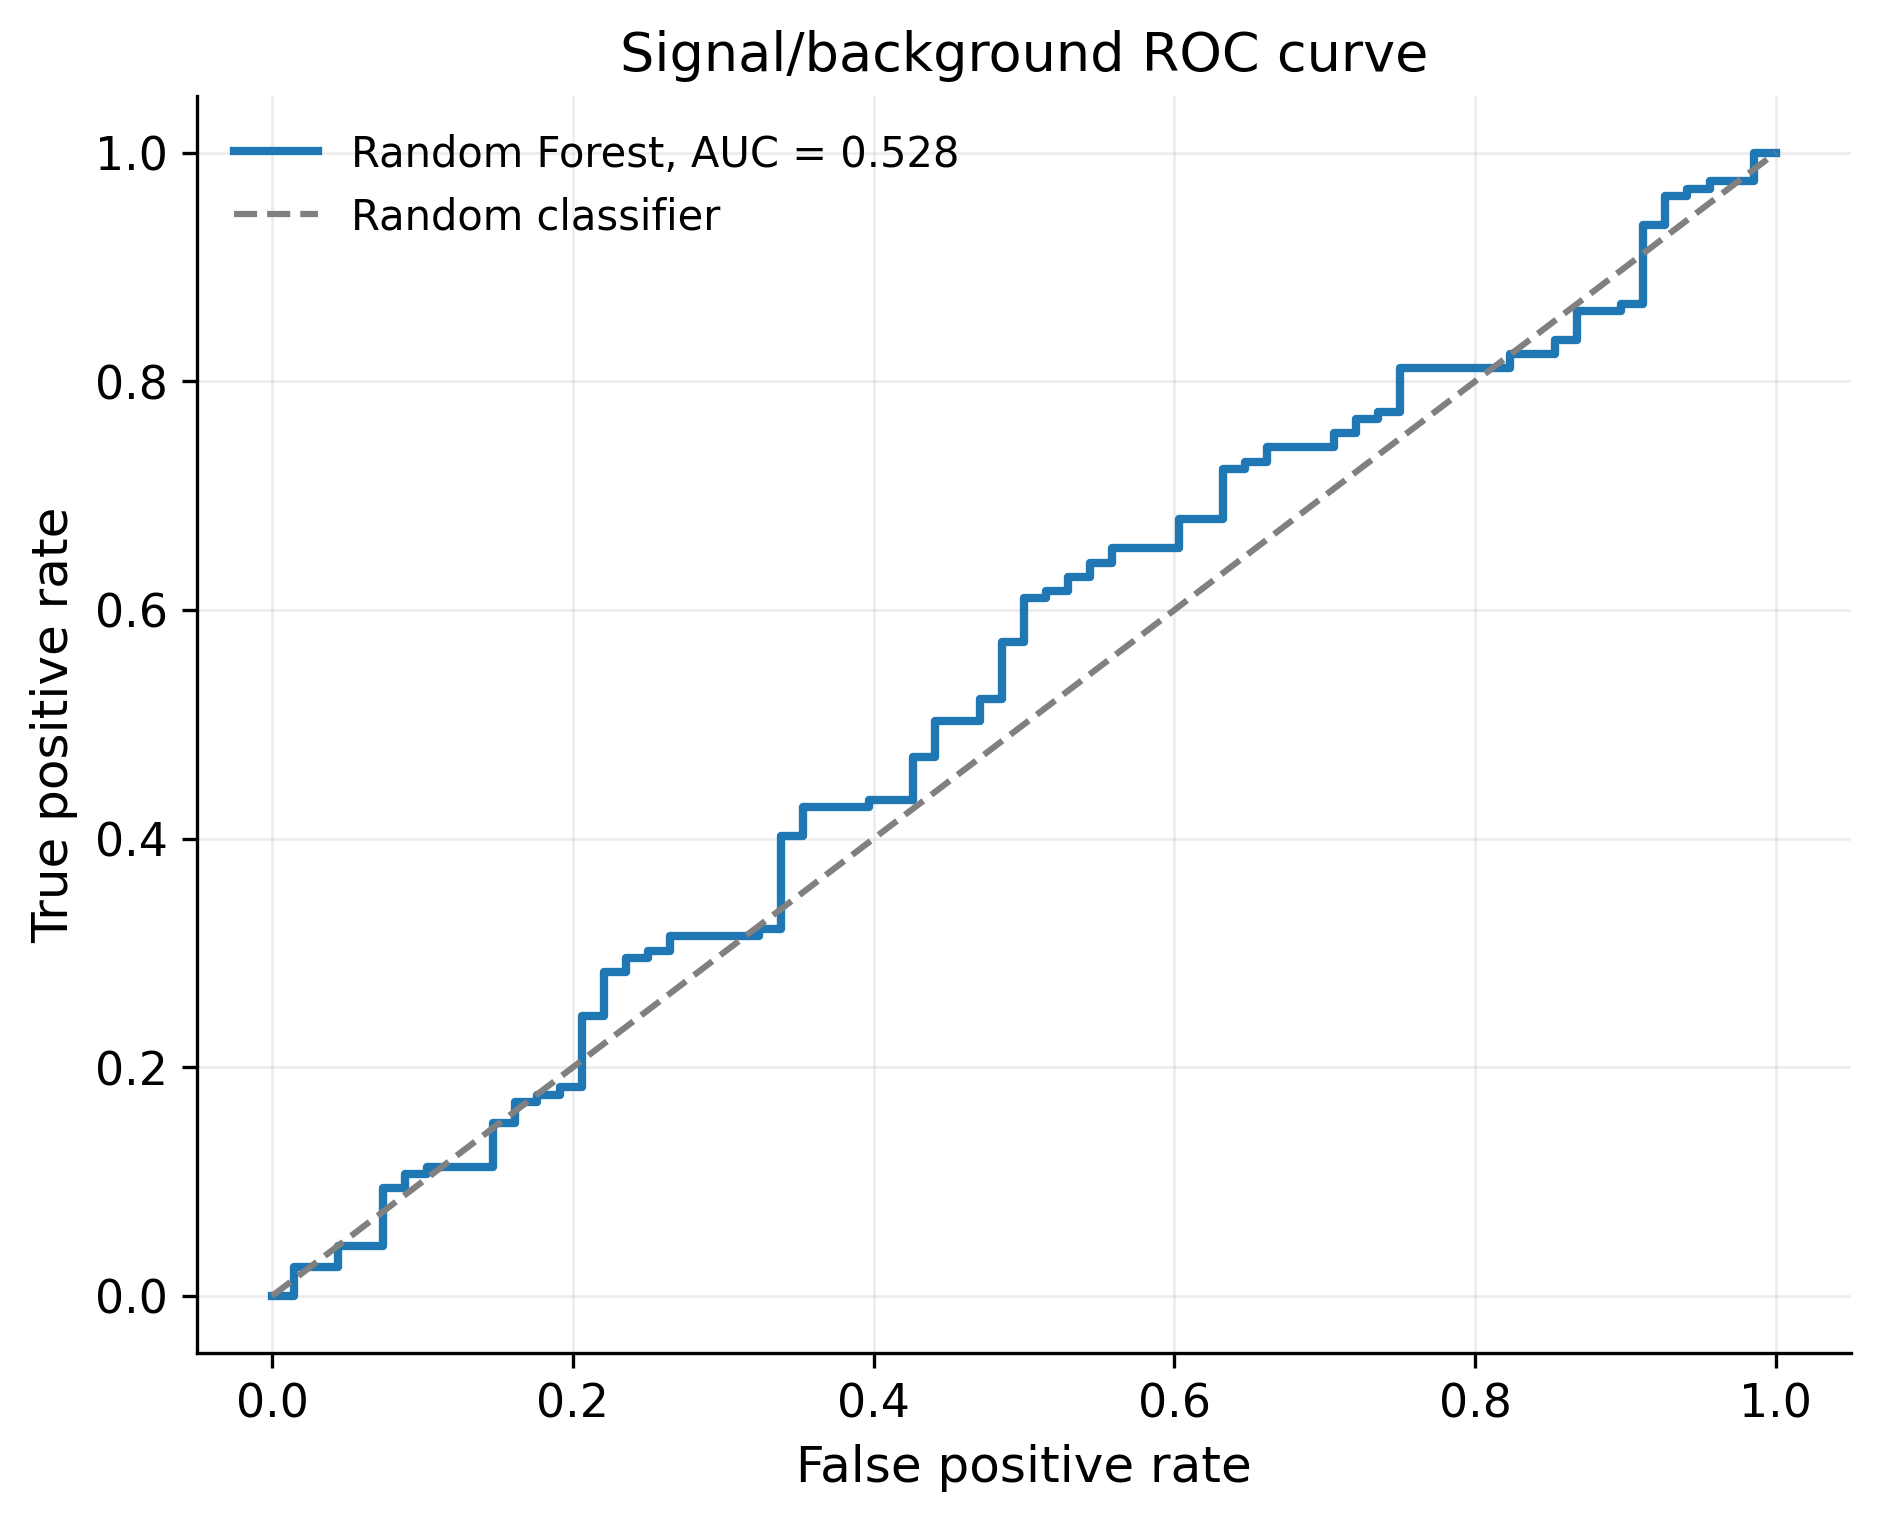
\includegraphics[width=0.75\textwidth]{roc_signal_background.png}
  \caption{ROC curve for the sideband-labelled Random Forest signal/background classifier.}
  \label{fig:roc}
\end{figure}

The measured area under the curve is $\mathrm{AUC}=0.528$. This is compatible
with no separation at all, and it should be read as a negative result rather than
as a performance figure. Two reasons explain it, and both are properties of the
analysis rather than of the algorithm. First, the baseline selection of
Sec.~\ref{sec:selection_effect} is already tight enough that the surviving sample
is dominated by signal; the classifier is asked to separate a background
population that has largely been removed. Second, the features available in the
ntuple are the same variables the selection already cuts on, so little
independent information is left. Training before the tight preselection, on a
looser sample and with additional kinematic variables, is the way to make this
study informative; it is listed as a planned extension.

Figure~\ref{fig:feature_importance} shows the feature-importance ranking from the Random Forest model. Given the AUC above, this ranking describes which variables the model used, not which variables carry physical discrimination. Such rankings depend on feature correlations, sample composition, and the chosen model architecture, and should not be read as physics observables.

\begin{figure}[H]
  \centering
  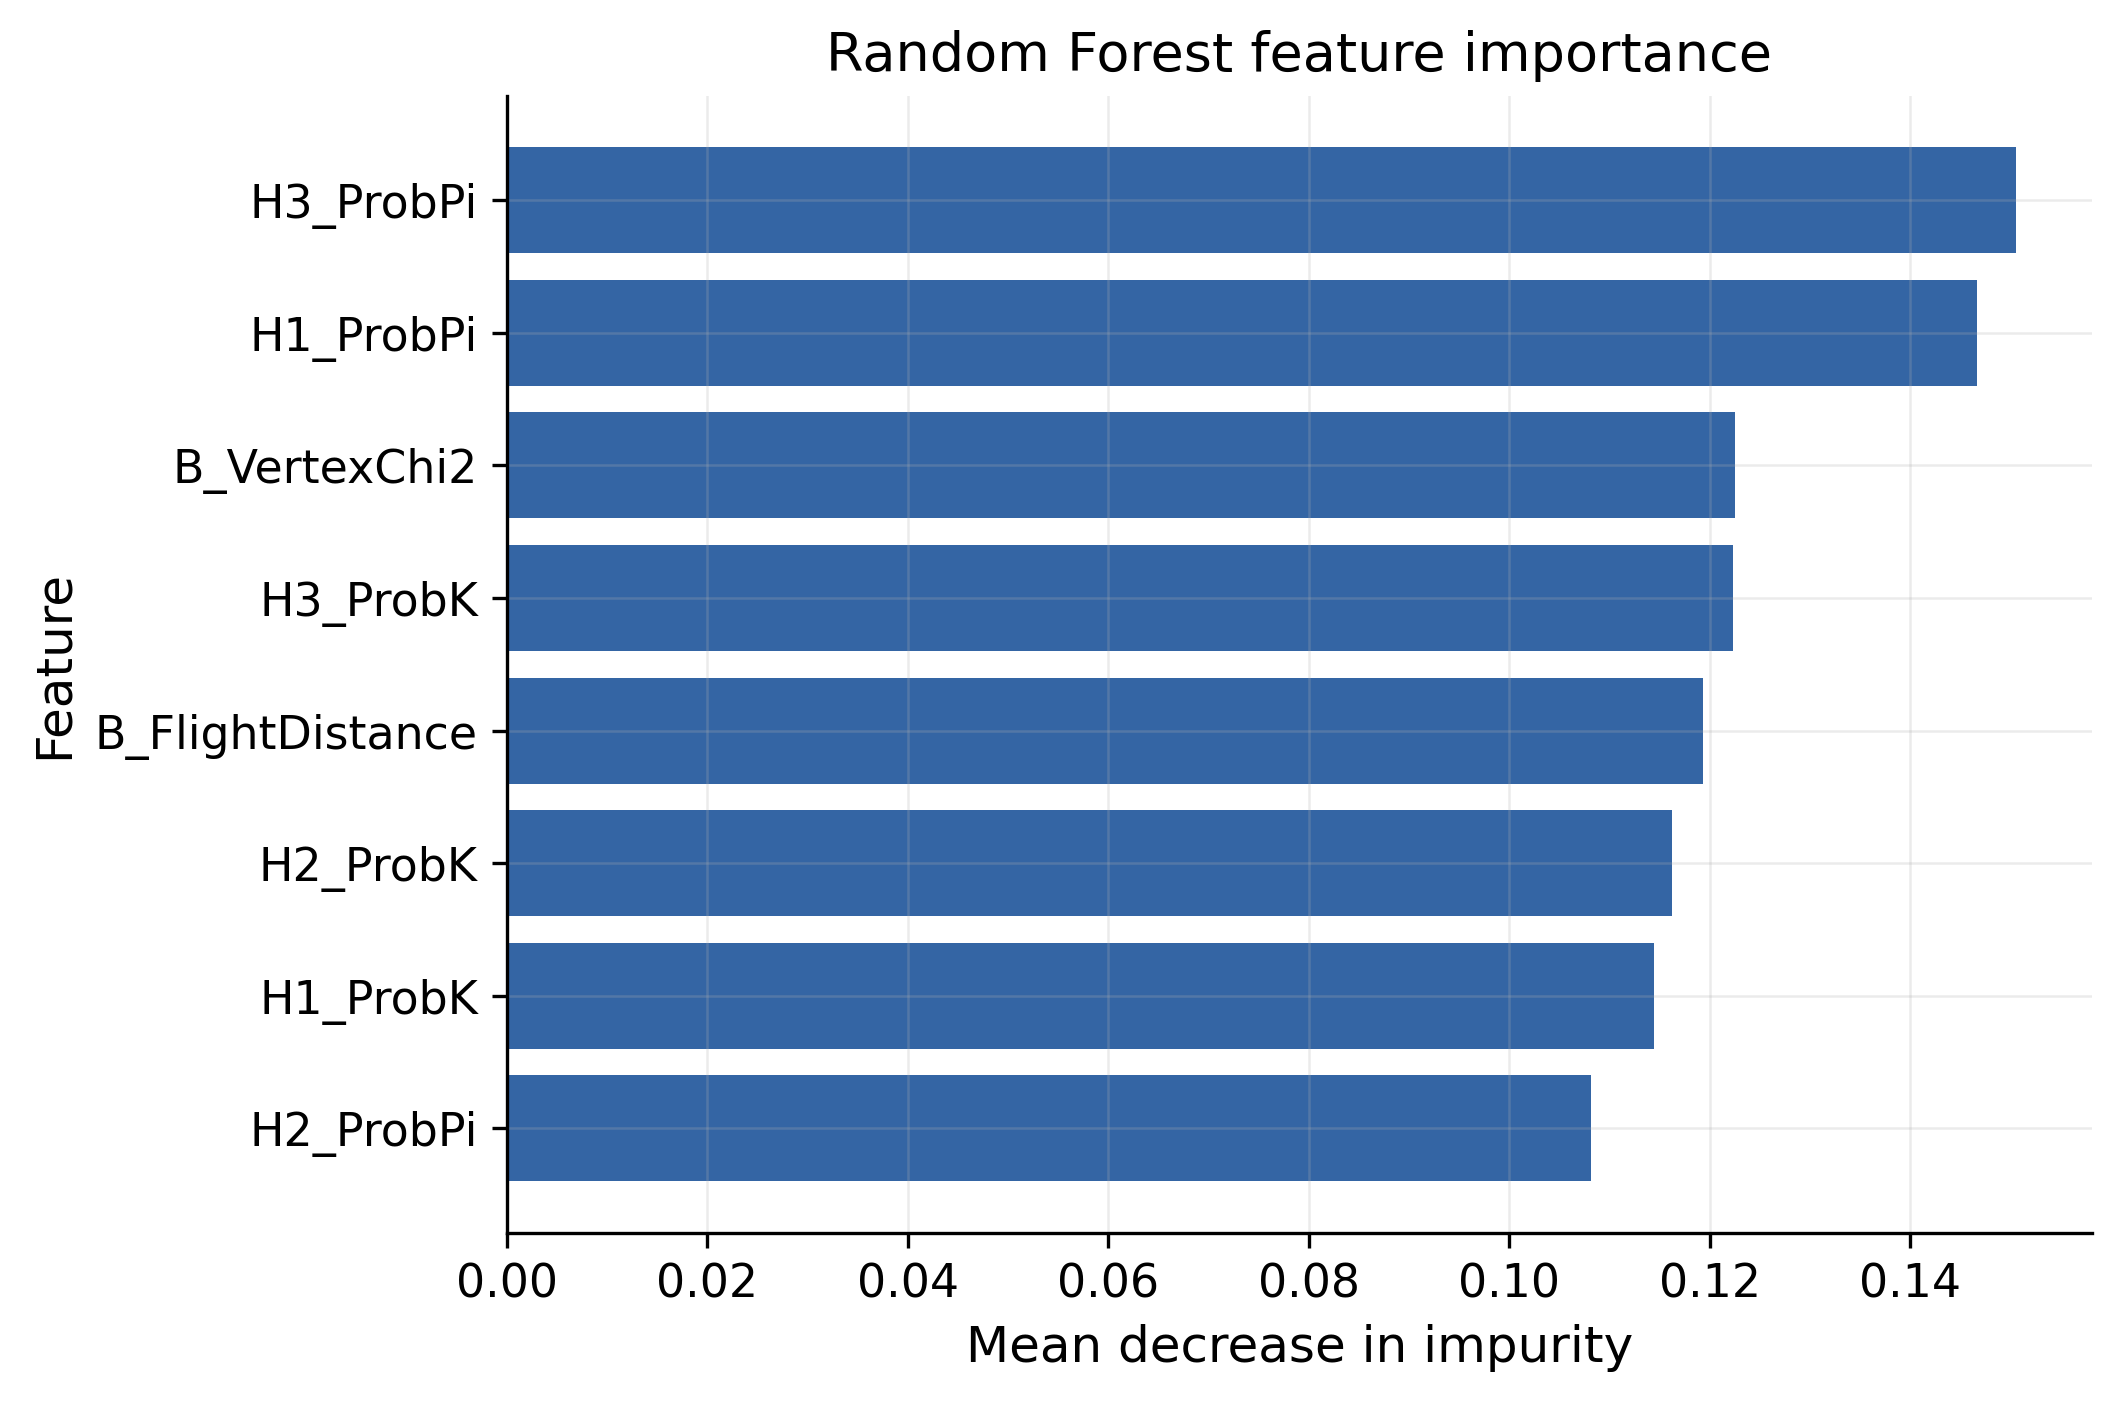
\includegraphics[width=0.82\textwidth]{feature_importance_signal_background.png}
  \caption{Random Forest feature importance for the signal/background classification task.}
  \label{fig:feature_importance}
\end{figure}

This part of the project demonstrates the integration of standard HEP sideband logic with modern machine-learning tools, and it also demonstrates when such a tool has nothing to add. The classifier is not used anywhere in the mass-fit, asymmetry or Dalitz results that follow; those rely on the transparent baseline selection alone. Making the classification study useful would require training before the preselection, cross-validation, gradient-boosted decision trees, systematic studies of the sideband definition, and comparisons with simulation.

\section{CP Asymmetry Study}

The selected candidates can be separated into charge-conjugate samples using the
total charge of the three daughter tracks,
\begin{equation}
  Q_{\mathrm{tot}} = Q(H_1) + Q(H_2) + Q(H_3).
\end{equation}
Candidates with $Q_{\mathrm{tot}}=+1$ are classified as \Bplus{} candidates,
while candidates with $Q_{\mathrm{tot}}=-1$ are classified as \Bminus{}
candidates. This assignment uses only reconstructed track-charge information
and is therefore a natural first step toward a charge-asymmetry study in a
three-charged-hadron final state.

\subsection{Charge-separated invariant-mass fits}

Rather than counting candidates in a fixed signal window, the updated
asymmetry extraction fits the \Bplus{} and \Bminus{} invariant-mass spectra
separately. Each charge sample is fitted in the range
$5000 < m(hhh) < 5600~\mevcc$ with a common-mean double-Gaussian signal model
and a finite-range exponential background model. The double-Gaussian signal
shape provides a narrow core plus a broader resolution component, which is a
more realistic detector-level description than a single Gaussian.

The fitted spectra are shown in Fig.~\ref{fig:charge_fit_plus} and
Fig.~\ref{fig:charge_fit_minus}. The fits converge for both charge categories
and give acceptable goodness-of-fit values, with
$\chi^2/\mathrm{ndof}=1.42$ for the \Bplus{} sample and
$\chi^2/\mathrm{ndof}=0.79$ for the \Bminus{} sample. The fitted signal yields
are
\begin{align}
  N(\Bplus) &= 694.4 \pm 27.2, \\
  N(\Bminus) &= 640.0 \pm 25.8,
\end{align}
where the uncertainties are the statistical yield uncertainties returned by
the binned mass fits.

\begin{figure}[H]
  \centering
  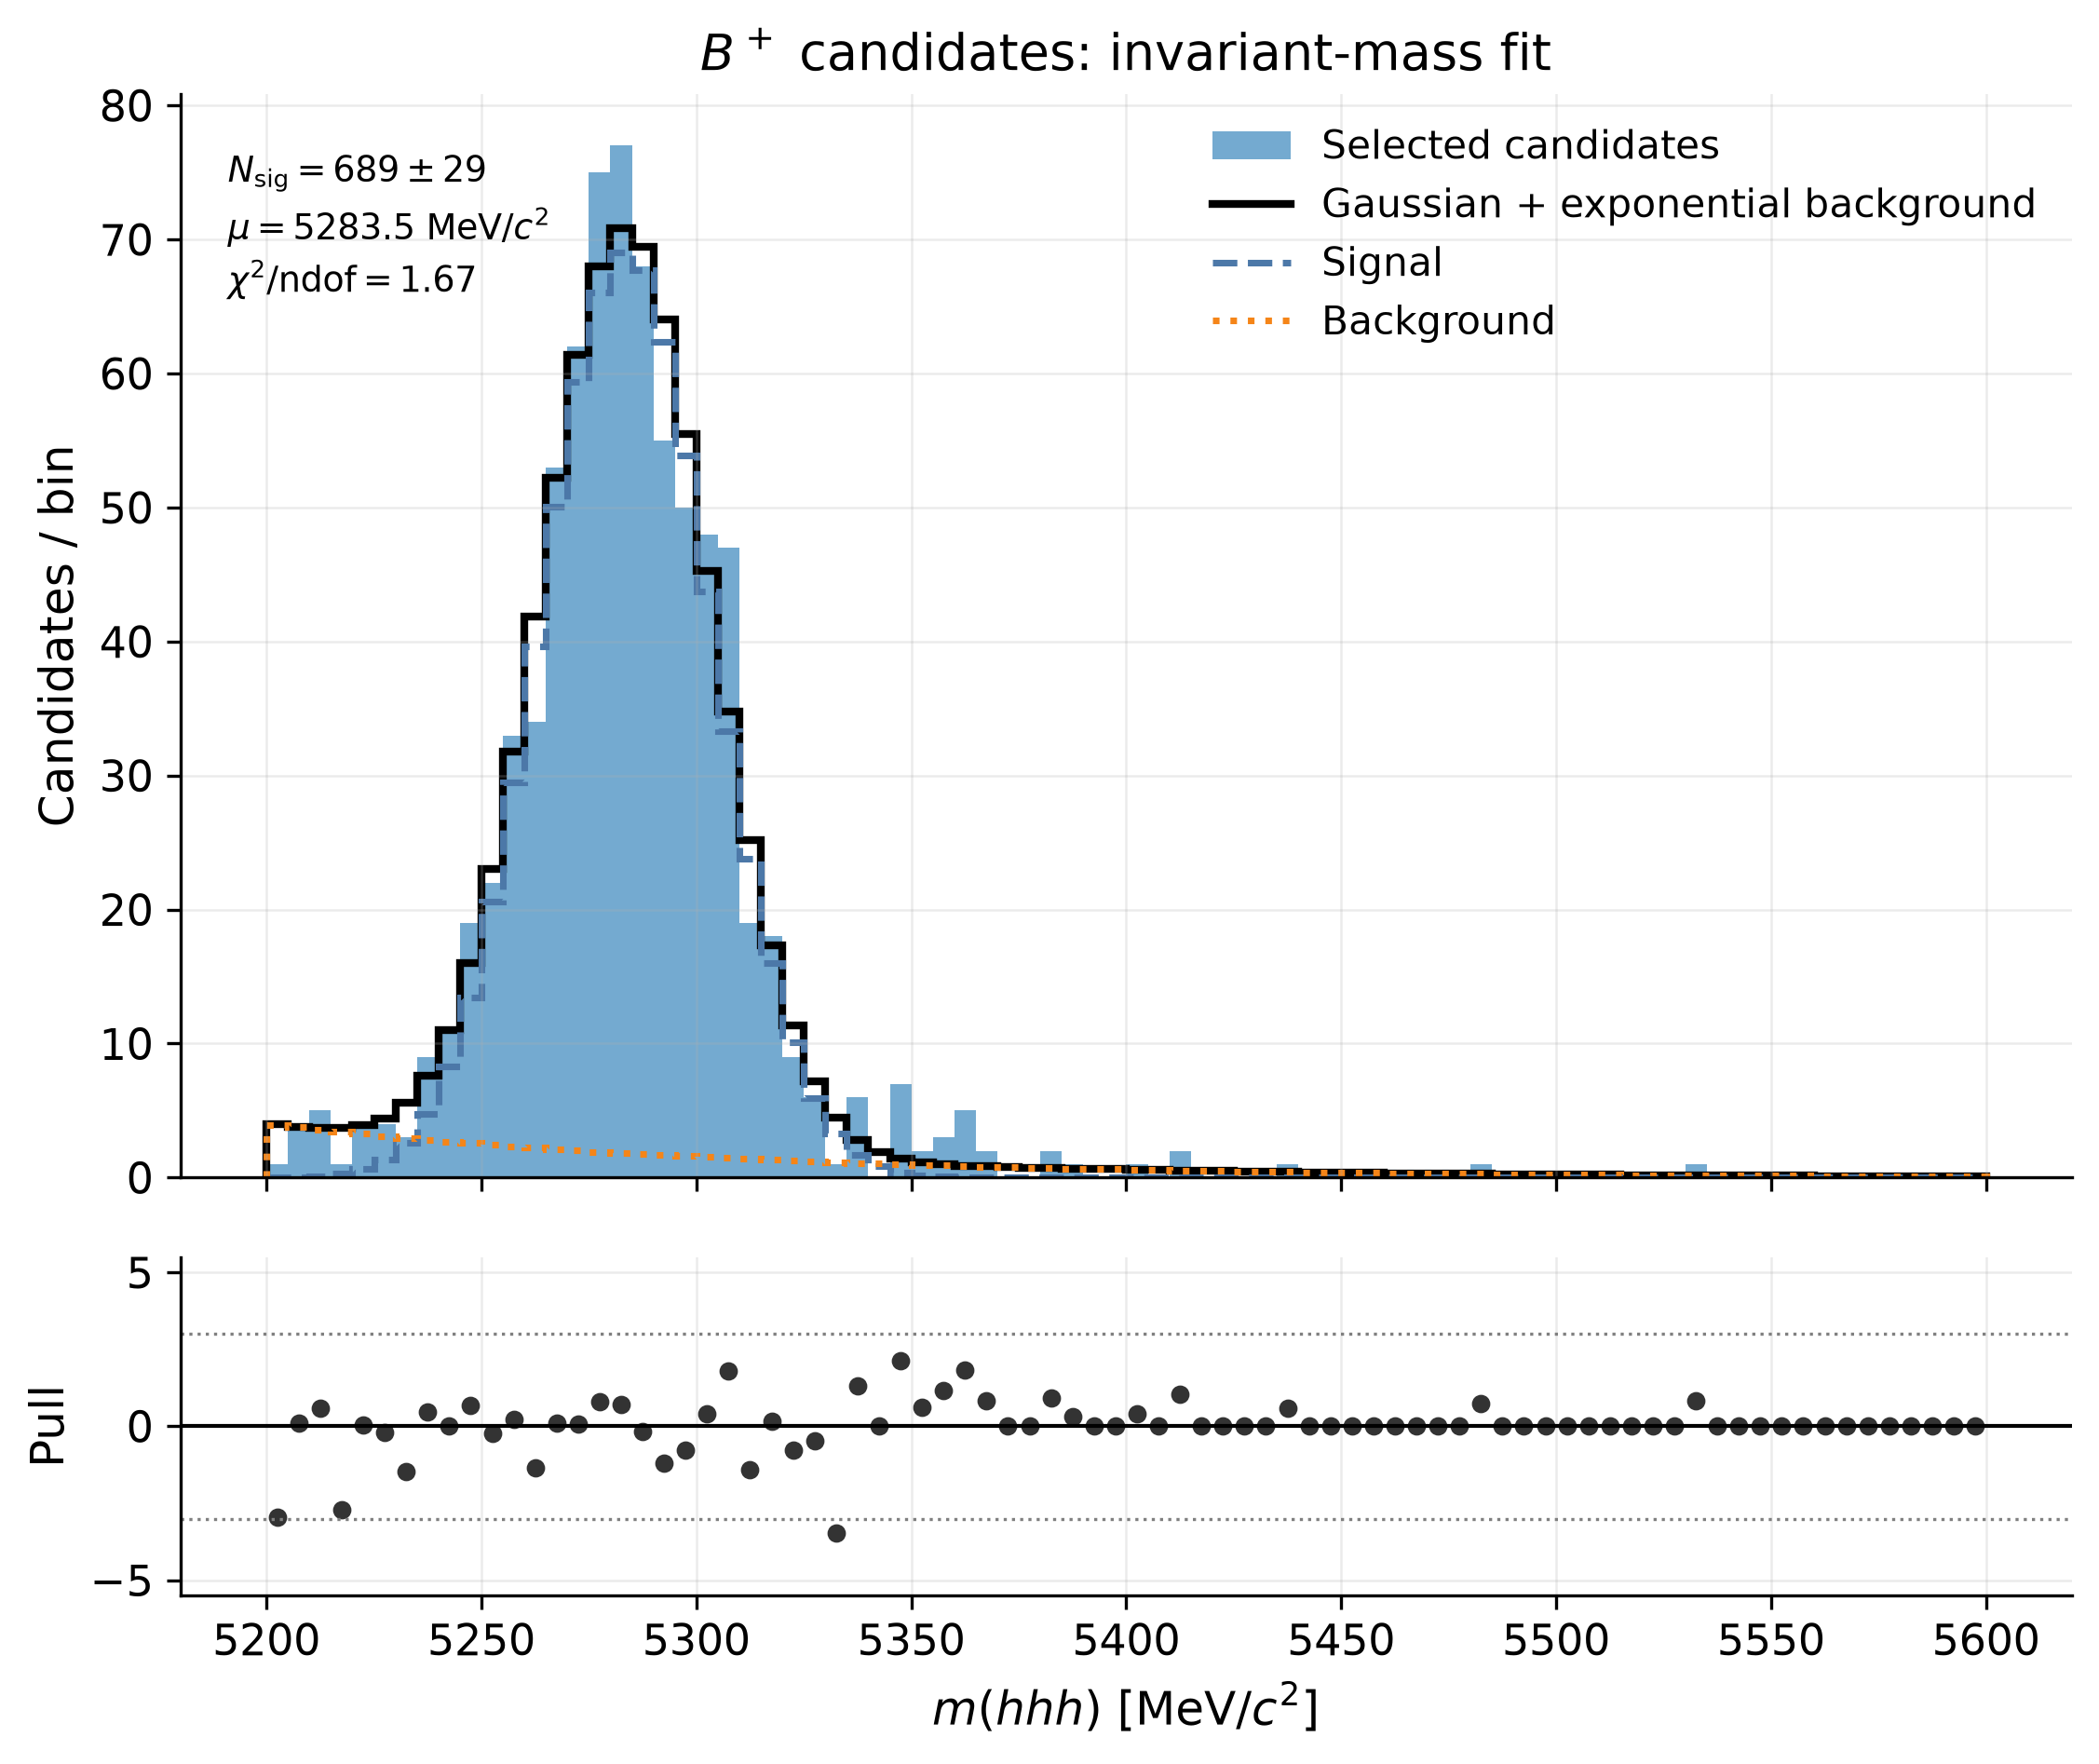
\includegraphics[width=0.82\textwidth]{B_plus_fit_plot.png}
  \caption{Charge-separated invariant-mass fit for the \Bplus{} candidate sample.}
  \label{fig:charge_fit_plus}
\end{figure}

\begin{figure}[H]
  \centering
  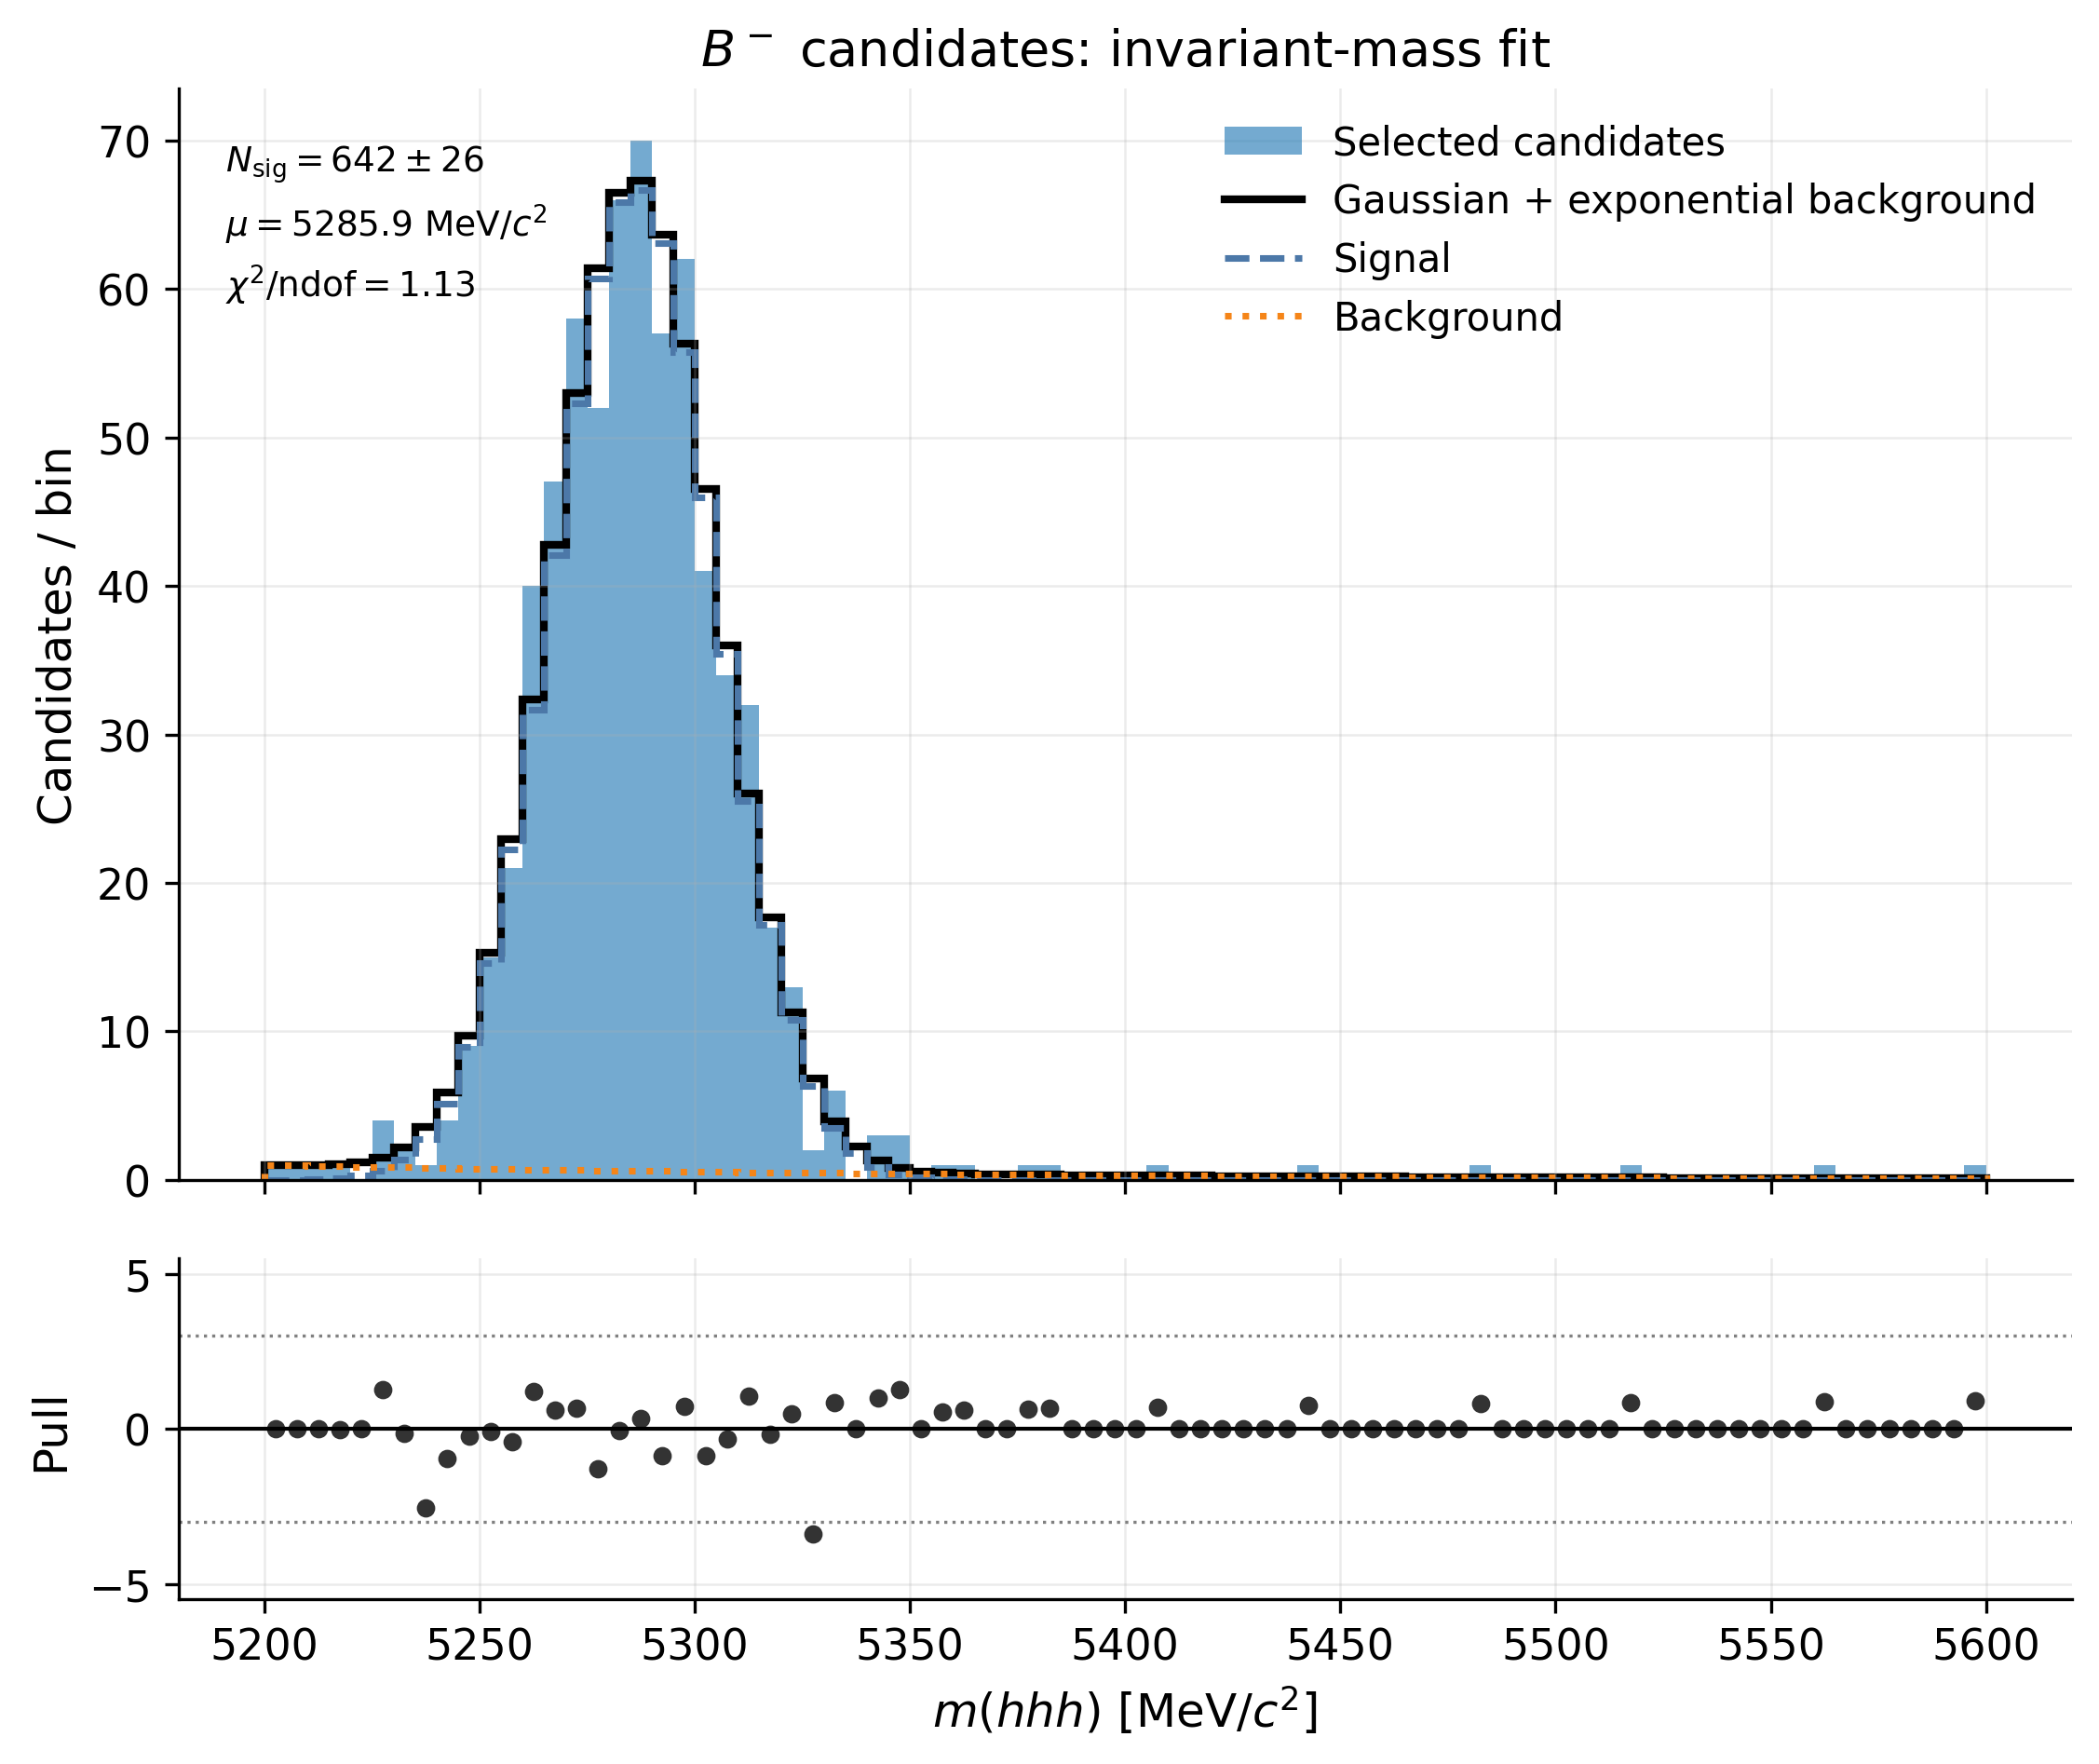
\includegraphics[width=0.82\textwidth]{B_minus_fit_plot.png}
  \caption{Charge-separated invariant-mass fit for the \Bminus{} candidate sample.}
  \label{fig:charge_fit_minus}
\end{figure}

\subsection{Raw asymmetry extraction}

The fitted signal yields are used to construct the raw asymmetry
\begin{equation}
  A_{\mathrm{raw}} =
  \frac{N(\Bminus)-N(\Bplus)}
       {N(\Bminus)+N(\Bplus)} .
  \label{eq:raw_asymmetry_fit}
\end{equation}
Propagating the independent fitted-yield uncertainties gives
\begin{equation}
  A_{\mathrm{raw}} = -0.0408 \pm 0.0281~\mathrm{(stat.)}.
\end{equation}
After including the systematic variations described below, the result is
reported as
\begin{equation}
  A_{\mathrm{raw}} =
  -0.0408 \pm 0.0281~\mathrm{(stat.)}
  \pm 0.0433~\mathrm{(syst.)}.
  \label{eq:raw_asymmetry_result}
\end{equation}

This is a raw asymmetry, not a physical CP-asymmetry measurement. It still
contains detector-induced charge asymmetries, possible \Bplus{}/\Bminus{}
production asymmetries, trigger and reconstruction effects, residual
background-model dependence, and selection-induced charge biases. A complete
measurement would require detector calibration, magnet-polarity combination,
background control, efficiency corrections, and a more complete systematic
uncertainty programme. The value in Eq.~\ref{eq:raw_asymmetry_result} should
therefore be interpreted as a diagnostic of the analysis workflow rather than
as evidence for CP violation.

\subsection{Toy-MC validation}

The statistical machinery was validated with pseudo-experiments generated from
the nominal charge-separated fitted model. In each toy experiment, \Bplus{} and
\Bminus{} mass spectra were generated with the injected fitted yields and then
refitted with the same double-Gaussian plus exponential model used in the data
fit. The toy study checks whether the fitting and uncertainty propagation
recover the injected raw asymmetry when the fit model is correct.

A 100-toy validation with fixed random seed produced 99 toys suitable for pull
studies and no fit failures. For the valid toys, the mean raw-asymmetry pull
was $-0.049$ and the pull width was $1.052$, compatible with the expected
standard normal behaviour for this sample size. The fitted bias was
$-0.0025$, well below the typical fitted statistical uncertainty of about
$0.029$. These results indicate that the nominal statistical extraction is
well behaved on pseudo-data generated from the fitted model. This validation is
not a detector-level systematic study.

\subsection{Systematic uncertainties}

Two first systematic categories are evaluated for the raw asymmetry: the choice
of mass-fit model and the choice of invariant-mass fit range. In both cases,
alternative fits are accepted only if the \Bplus{} and \Bminus{} fits converge,
the fitted yields and yield uncertainties are positive, and the
$\chi^2/\mathrm{ndof}$ values remain below 2.5 for both charge-separated mass
spectra.

The fit-model study compares the nominal double-Gaussian plus exponential model
with an accepted double-Gaussian plus linear-background alternative. A
single-Gaussian plus exponential model is also retained as a stress test, but
it is not used to assign the systematic uncertainty because it does not provide
an acceptable description of the \Bminus{} spectrum. The accepted
linear-background variation shifts the raw asymmetry by $0.0255$, which is
taken as the fit-model systematic uncertainty.

\begin{figure}[H]
  \centering
  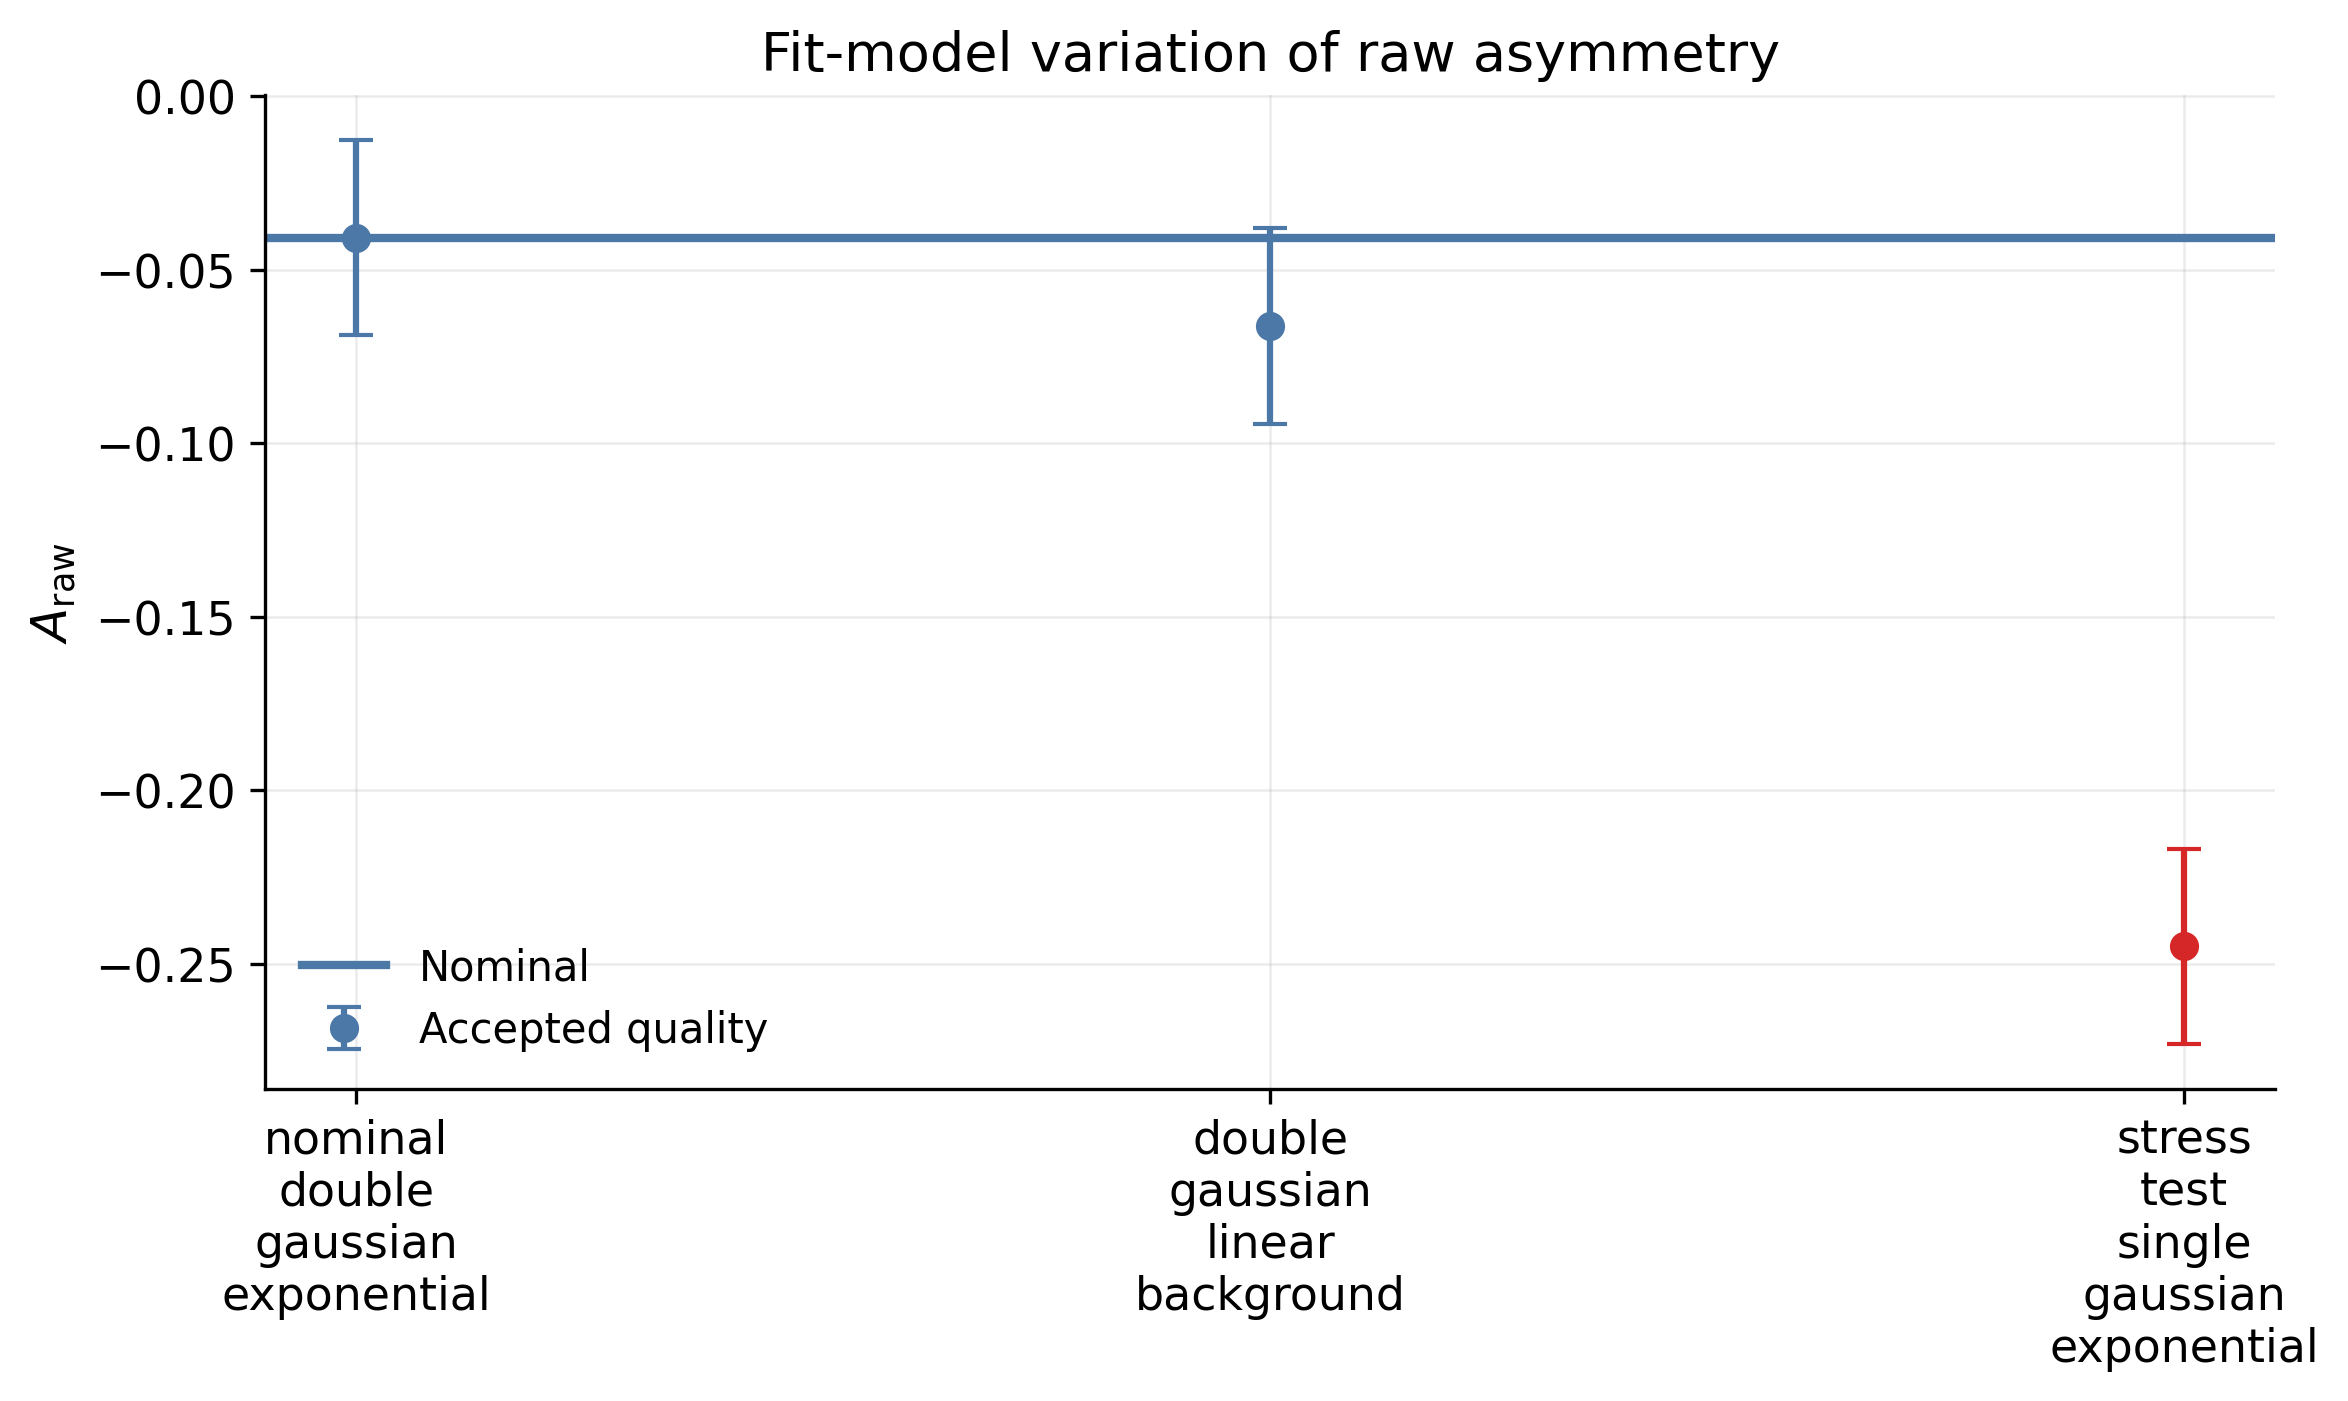
\includegraphics[width=0.82\textwidth]{fit_model_variations.png}
  \caption{Raw asymmetry obtained with different charge-separated mass-fit models. Rejected stress-test variations are shown for comparison but are not used in the systematic assignment.}
  \label{fig:fit_model_systematic}
\end{figure}

The fit-range study repeats the nominal double-Gaussian plus exponential fits
for narrower and wider mass intervals. These variations test the sensitivity
to the amount of sideband information included in the background constraint.
All tested fit-range variations pass the quality requirements. The largest
accepted shift is $0.0350$, obtained from the wider high-mass range
$5000 < m(hhh) < 5700~\mevcc$, and is assigned as the fit-range systematic
uncertainty.

\begin{figure}[H]
  \centering
  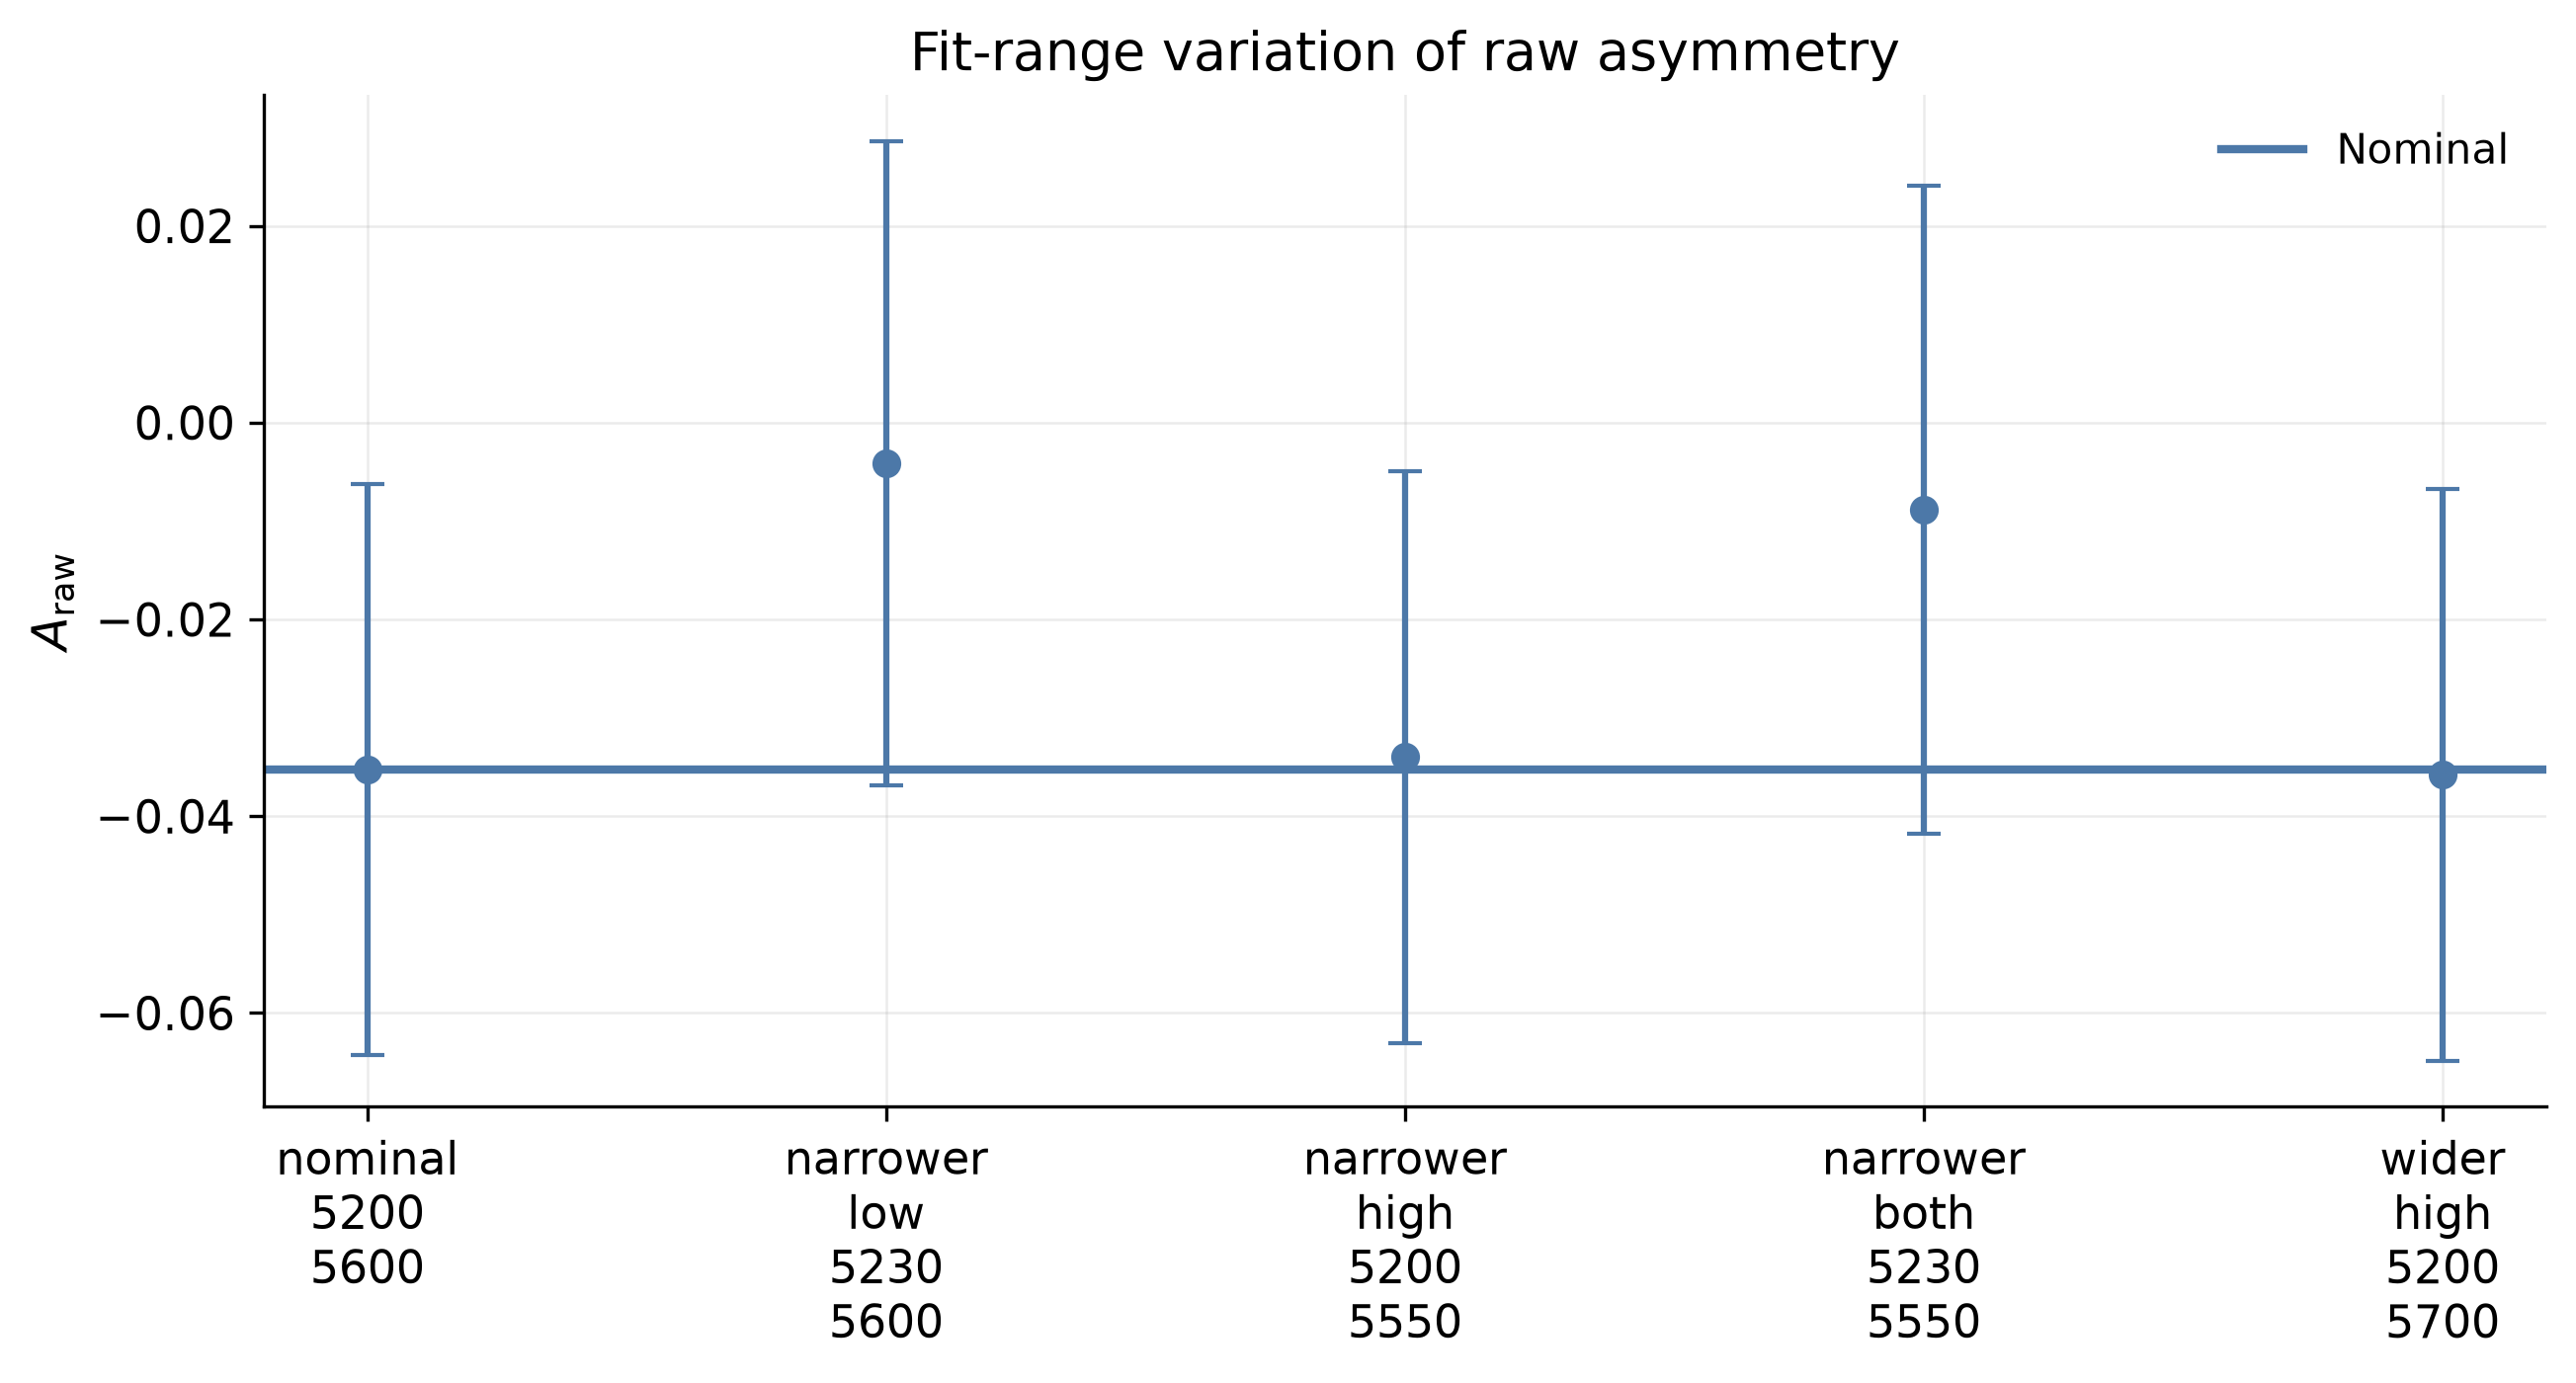
\includegraphics[width=0.82\textwidth]{fit_range_variations.png}
  \caption{Raw asymmetry obtained for alternative invariant-mass fit ranges using the nominal signal and background model.}
  \label{fig:fit_range_systematic}
\end{figure}

Table~\ref{tab:raw_asymmetry_uncertainties} summarizes the uncertainty
components. The total systematic uncertainty is obtained by adding the
fit-model and fit-range components in quadrature. The total uncertainty,
including statistics, is $0.0516$.

\begin{table}[H]
  \centering
  \caption{Uncertainty components for the fitted raw asymmetry.}
  \label{tab:raw_asymmetry_uncertainties}
  \begin{tabular}{lc}
    \toprule
    Source & Uncertainty on $A_{\mathrm{raw}}$ \\
    \midrule
    Statistical & 0.0281 \\
    Fit-model systematic & 0.0255 \\
    Fit-range systematic & 0.0350 \\
    Total systematic & 0.0433 \\
    \bottomrule
  \end{tabular}
\end{table}

\begin{figure}[H]
  \centering
  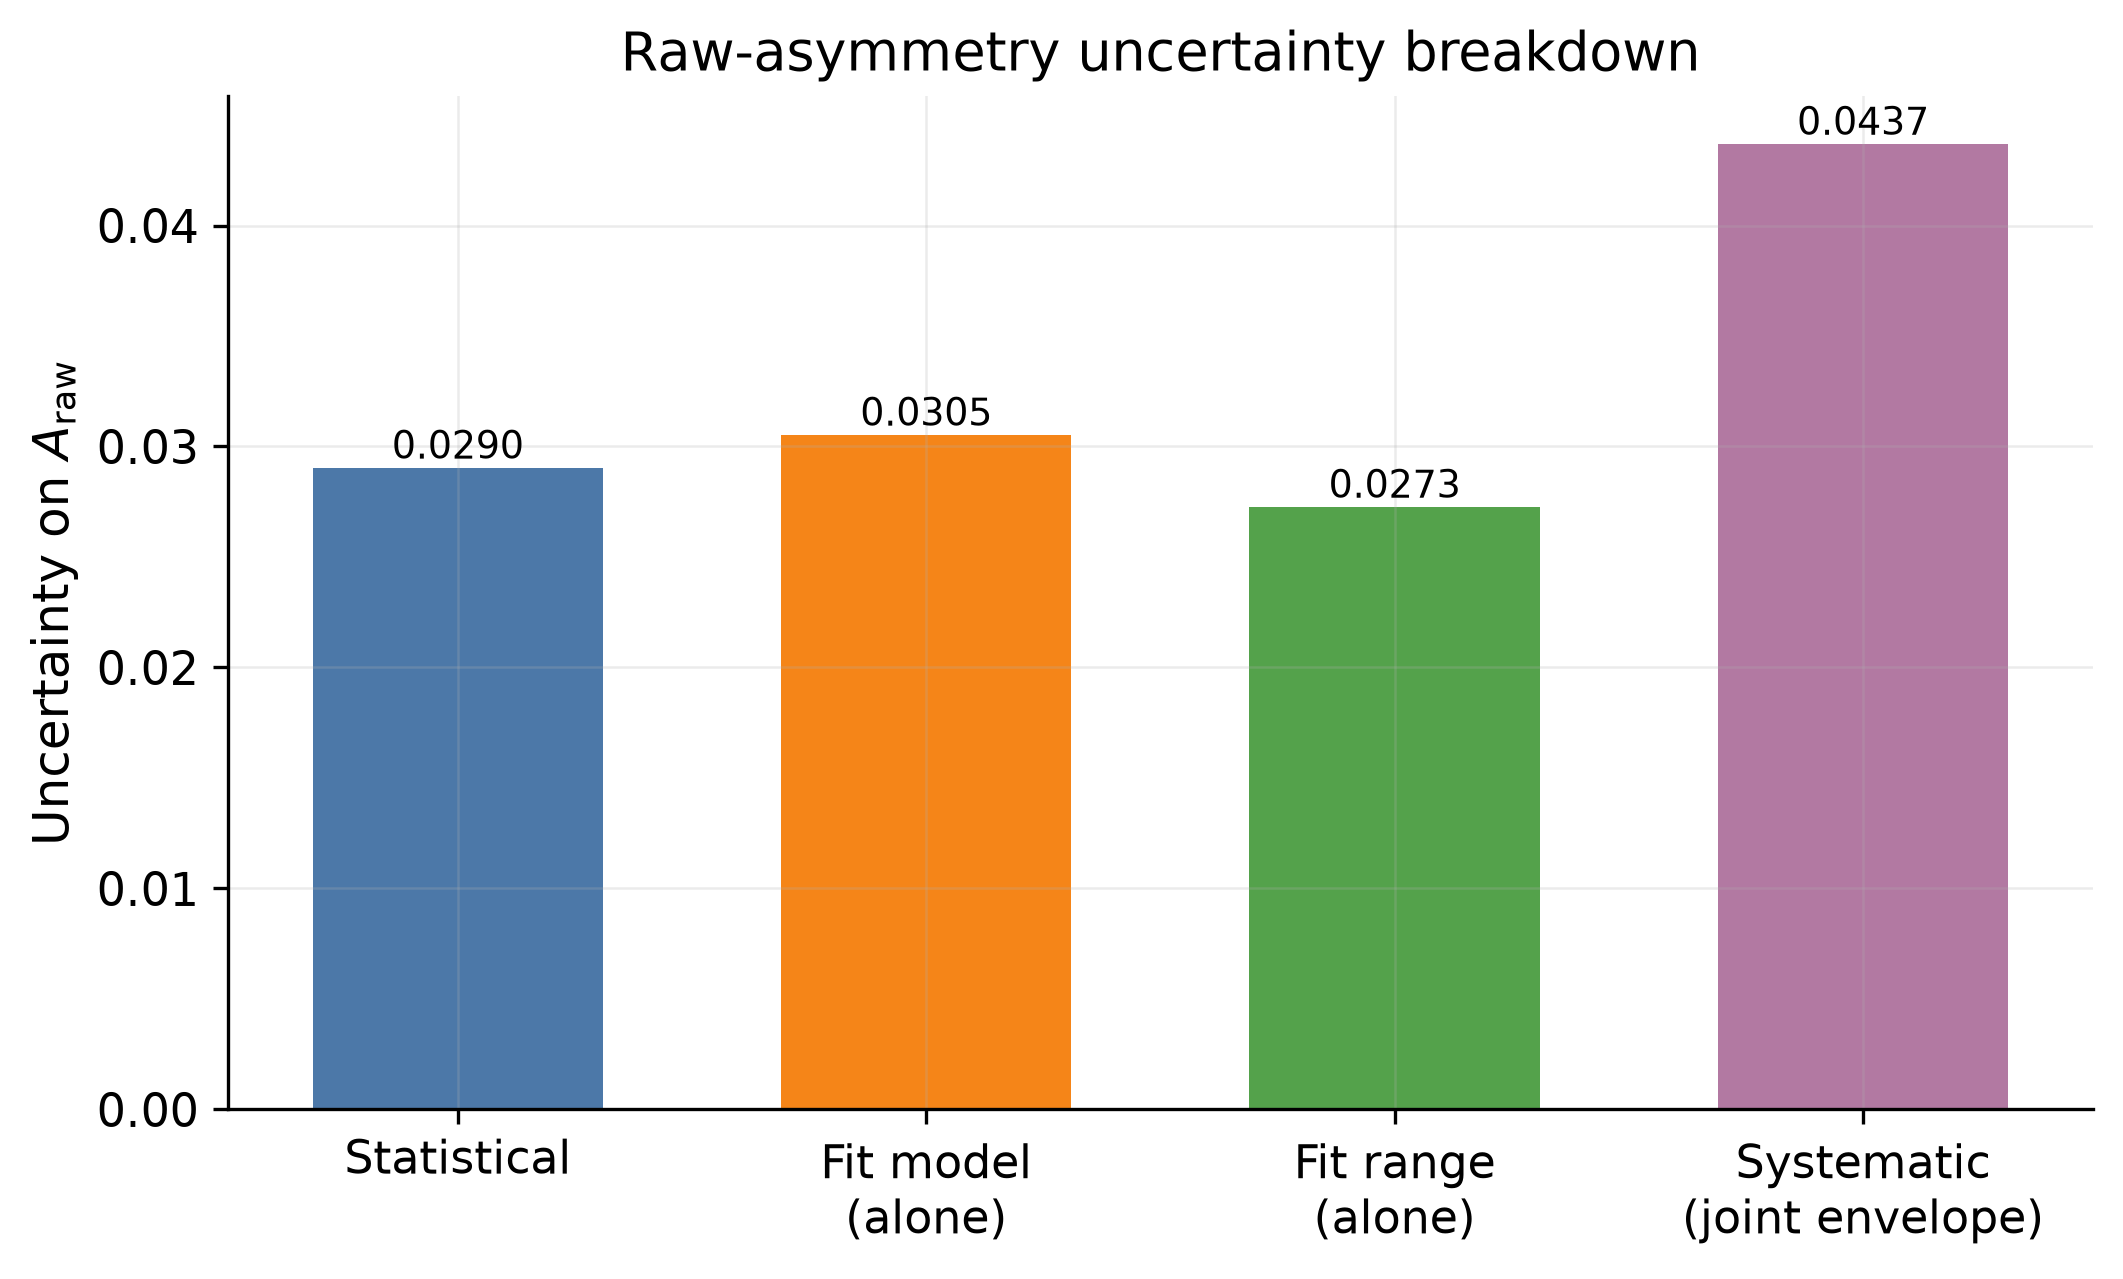
\includegraphics[width=0.72\textwidth]{systematic_breakdown.png}
  \caption{Breakdown of the statistical uncertainty, individual systematic components, and total systematic uncertainty on the raw asymmetry.}
  \label{fig:systematic_breakdown}
\end{figure}

The dominant systematic contribution in this first study comes from the fit
range, followed by the background-model variation. These studies probe only a
limited set of analysis choices. Additional signal-shape variations, broader
background-shape alternatives, magnet-polarity comparisons, and
detector-efficiency corrections would be required before interpreting the raw
asymmetry as a corrected CP observable.

\clearpage

\section{Dalitz Plot Analysis}

\subsection{Pairwise invariant masses}

Three-body decays contain more kinematic information than a single reconstructed parent mass. The internal phase-space structure can be studied using pairwise invariant masses. For three daughter tracks labelled $K_1$, $K_2$, and $K_3$, the Dalitz variables used in this project are
\begin{align}
  m^2(K_1K_2), \qquad
  m^2(K_2K_3), \qquad
  m^2(K_1K_3).
\end{align}
Only two of these variables are independent for a fixed parent mass, but plotting different pairs is useful for visual inspection and for checking symmetries or structures involving different track orderings.

The pair mass is computed by summing the two daughter four-vectors:
\begin{equation}
  m_{ij}^2 =
  \left(E_i + E_j\right)^2
  -
  \left|\vec{p}_i + \vec{p}_j\right|^2 .
\end{equation}
As in the B-mass reconstruction, each daughter is assigned the kaon mass hypothesis. The resulting squared masses are reported in \gevfour{} to keep the numerical axis scales readable.

\subsection{Dalitz distributions and resonance structure}

A Dalitz plot displays the density of selected events in a two-dimensional plane of pairwise invariant-mass-squared variables. Resonant two-body substructures can appear as bands, while interference and phase-space effects can produce non-uniform densities. In a complete amplitude analysis, these structures would be modelled with coherent sums of resonant and non-resonant amplitudes. The present analysis restricts itself to visualising the distributions.

Figure~\ref{fig:dalitz_12_23} shows the distribution in the $m^2(K_1K_2)$ versus $m^2(K_2K_3)$ plane. The use of a two-dimensional histogram rather than a raw scatter plot makes dense regions easier to read.

\begin{figure}[H]
  \centering
  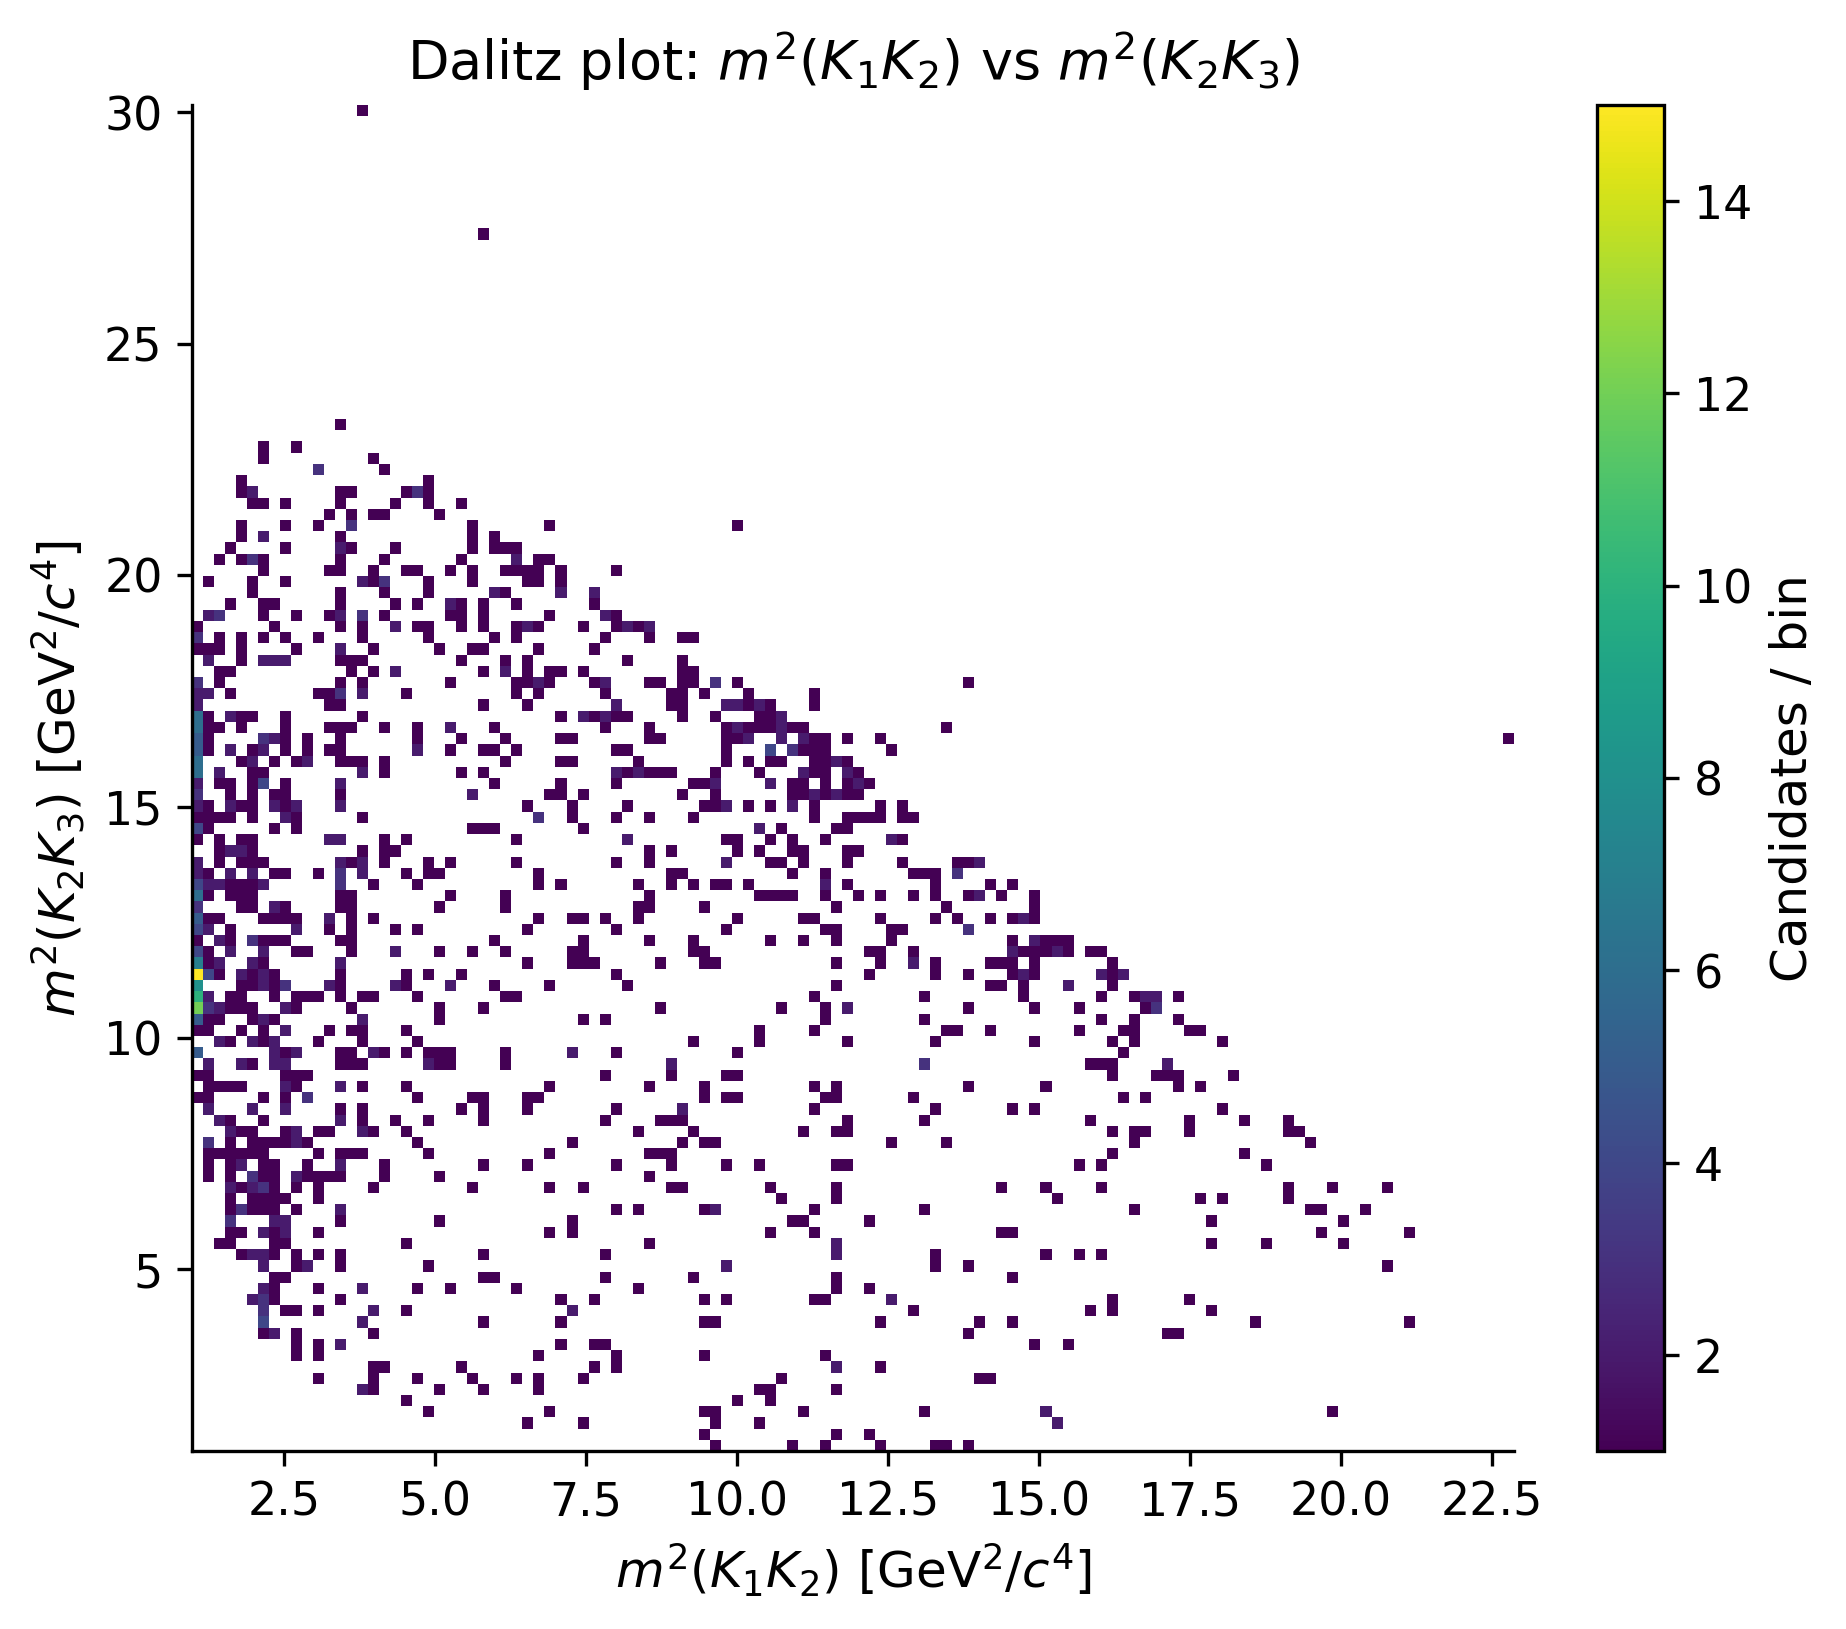
\includegraphics[width=0.78\textwidth]{dalitz_mK1K2_vs_mK2K3.png}
  \caption{Dalitz density map in the $m^2(K_1K_2)$ versus $m^2(K_2K_3)$ plane.}
  \label{fig:dalitz_12_23}
\end{figure}

Figures~\ref{fig:dalitz_12_13} and~\ref{fig:dalitz_23_13} show the complementary pairings. Together, these projections provide a first view of the three-body phase-space population after the baseline selection.

\begin{figure}[H]
  \centering
  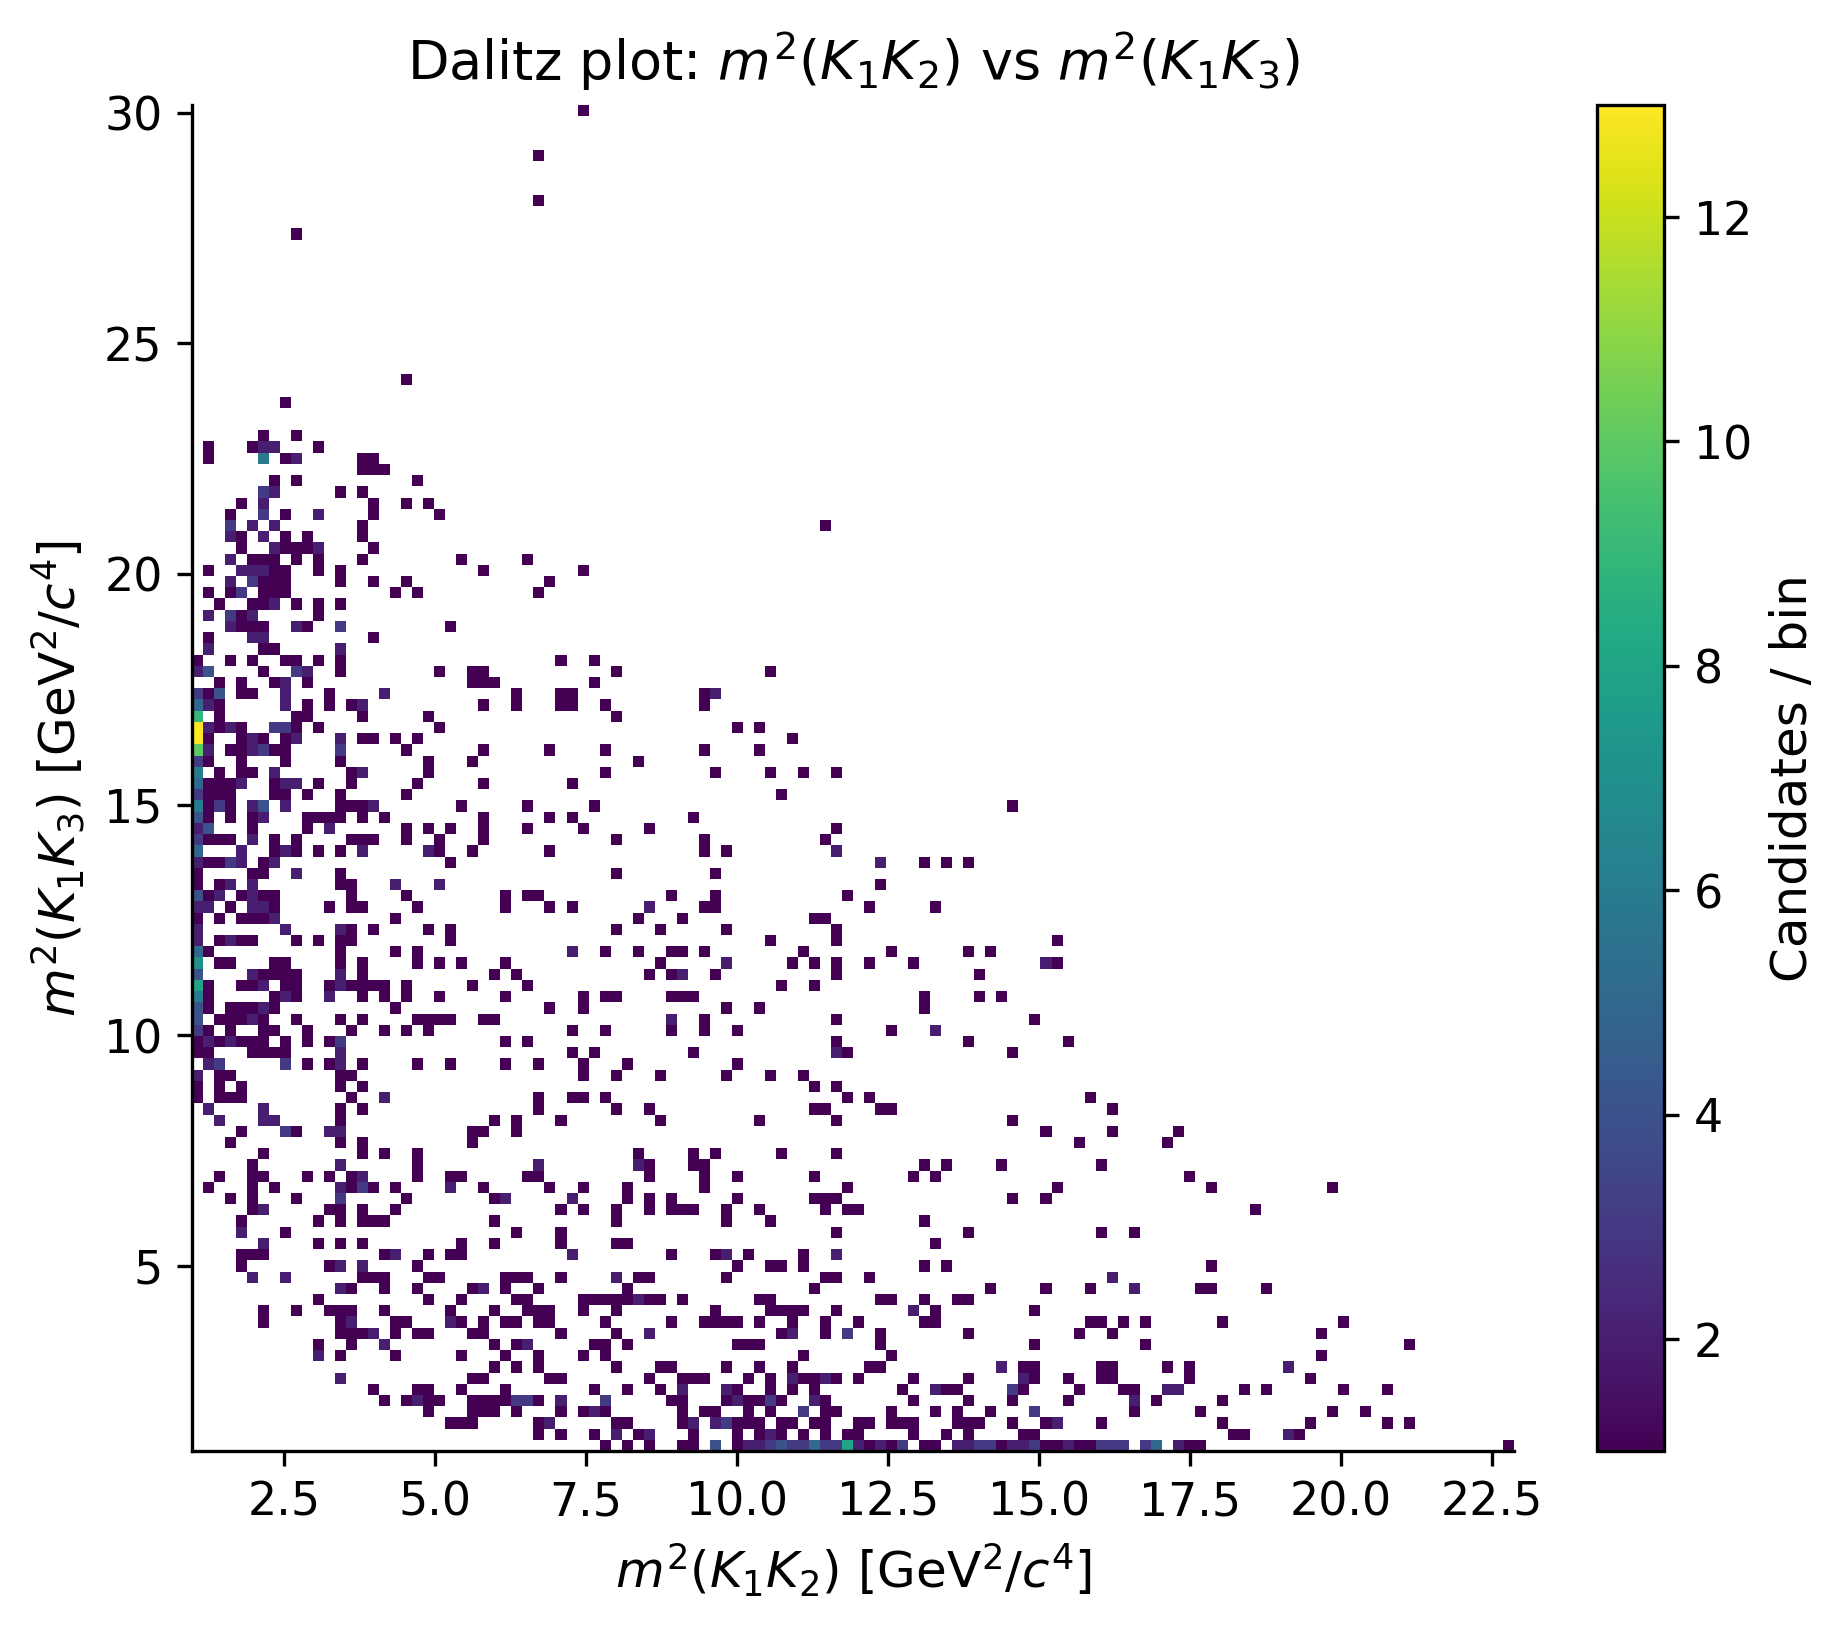
\includegraphics[width=0.78\textwidth]{dalitz_mK1K2_vs_mK1K3.png}
  \caption{Dalitz density map in the $m^2(K_1K_2)$ versus $m^2(K_1K_3)$ plane.}
  \label{fig:dalitz_12_13}
\end{figure}

\begin{figure}[H]
  \centering
  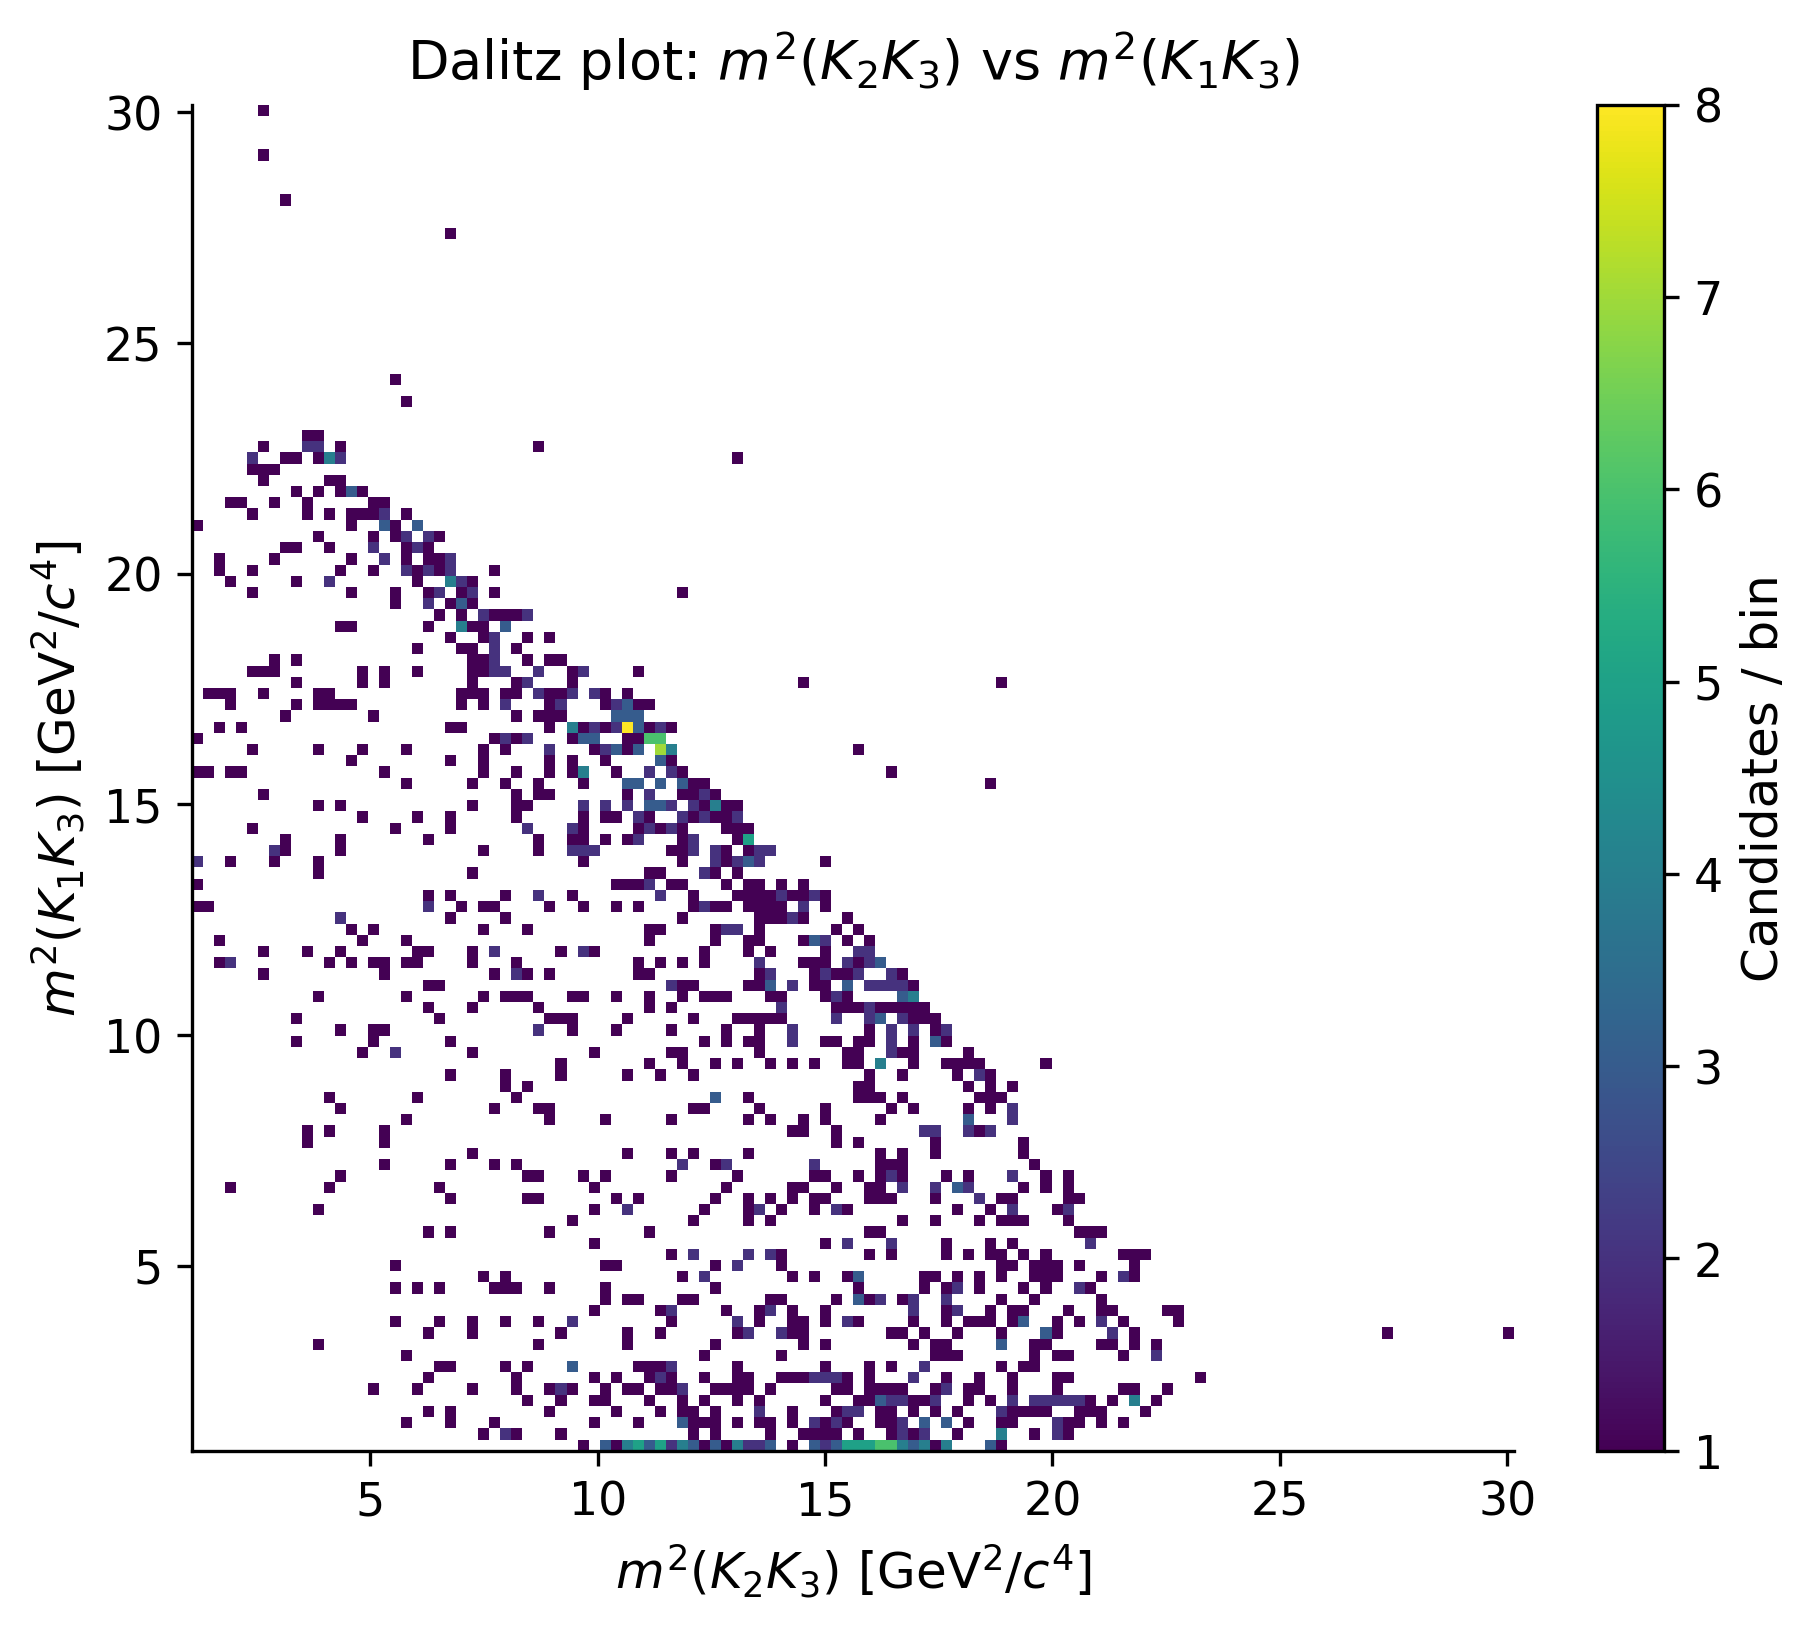
\includegraphics[width=0.78\textwidth]{dalitz_mK2K3_vs_mK1K3.png}
  \caption{Dalitz density map in the $m^2(K_2K_3)$ versus $m^2(K_1K_3)$ plane.}
  \label{fig:dalitz_23_13}
\end{figure}

Dalitz plots are especially relevant for CP-violation studies in multibody decays. Even if the integrated raw asymmetry is small, local asymmetries in restricted phase-space regions can be larger. A natural future extension would therefore compare the Dalitz distributions of \Bplus{} and \Bminus{} candidates, using background subtraction and detector-efficiency corrections.

\section{Conclusion}

This project demonstrates a complete and modern introductory HEP analysis workflow using LHCb CERN Open Data. Starting from ROOT ntuples, the analysis reads selected branches with \texttt{uproot}, processes candidates with \texttt{pandas} and \texttt{numpy}, reconstructs invariant masses, applies physics-motivated selections, generates publication-style plots, trains a sideband-labelled Random Forest classifier, performs charge-separated invariant-mass fits, computes a raw charge asymmetry, and visualises three-body phase space with Dalitz plots.

The invariant-mass reconstruction shows a clear B-candidate peak after the baseline selection. The selected mass spectrum is described with a double-Gaussian signal model and an exponential background model, providing a realistic detector-level signal extraction framework. The signal/background classification study demonstrates how sideband labels can be combined with standard machine-learning tools, while the ROC curve and feature-importance plot provide useful performance diagnostics. The CP-asymmetry study separates \Bplus{} and \Bminus{} candidates, performs independent invariant-mass fits, and extracts a raw integrated asymmetry together with statistical and systematic uncertainty estimates. Toy-MC pseudo-experiments are used to validate the statistical behaviour of the fitting procedure and uncertainty propagation. The Dalitz analysis extends the project toward multibody-decay phase-space studies by reconstructing pairwise invariant-mass-squared variables.

The analysis remains intentionally simplified and does not constitute a precision flavour-physics measurement. Several improvements would still be required for a full experimental analysis:
\begin{itemize}
  \item train stronger classifiers such as XGBoost or gradient-boosted decision trees, with cross-validation and robust overtraining checks;
  \item include detector effects, PID calibration, trigger efficiencies, and reconstruction asymmetries;
  \item use simulation and control samples to validate selection efficiencies and background shapes;
  \item combine MagnetUp and MagnetDown samples to reduce charge-dependent detector biases;
  \item implement additional accepted fit-model variations, such as Crystal Ball signal models or alternative background parameterisations;
  \item perform local CP-asymmetry studies across Dalitz-plot regions.
\end{itemize}

Despite these limitations, the project captures several essential components of a realistic experimental-particle-physics analysis: transparent event reconstruction, documented selection choices, modular code, reproducible figures, signal extraction through invariant-mass fitting, uncertainty propagation, toy-MC validation, and explicit treatment of systematic effects. It therefore provides a strong foundation for more advanced studies in heavy-flavour physics and for future work in an experimental PhD environment.

\newpage
\bibliographystyle{unsrt}
\bibliography{bibliography}

\end{document}
